\documentclass[]{article}
\usepackage{lmodern}
\usepackage{amssymb,amsmath}
\usepackage{ifxetex,ifluatex}
\usepackage{fixltx2e} % provides \textsubscript
\ifnum 0\ifxetex 1\fi\ifluatex 1\fi=0 % if pdftex
  \usepackage[T1]{fontenc}
  \usepackage[utf8]{inputenc}
\else % if luatex or xelatex
  \ifxetex
    \usepackage{mathspec}
  \else
    \usepackage{fontspec}
  \fi
  \defaultfontfeatures{Ligatures=TeX,Scale=MatchLowercase}
\fi
% use upquote if available, for straight quotes in verbatim environments
\IfFileExists{upquote.sty}{\usepackage{upquote}}{}
% use microtype if available
\IfFileExists{microtype.sty}{%
\usepackage{microtype}
\UseMicrotypeSet[protrusion]{basicmath} % disable protrusion for tt fonts
}{}
\usepackage[margin=1in]{geometry}
\usepackage{hyperref}
\hypersetup{unicode=true,
            pdftitle={Web-based Supplementary Materials for The Effect of Recycled Individuals in the Jolly-Seber Tag Loss Model},
            pdfborder={0 0 0},
            breaklinks=true}
\urlstyle{same}  % don't use monospace font for urls
\usepackage{graphicx,grffile}
\makeatletter
\def\maxwidth{\ifdim\Gin@nat@width>\linewidth\linewidth\else\Gin@nat@width\fi}
\def\maxheight{\ifdim\Gin@nat@height>\textheight\textheight\else\Gin@nat@height\fi}
\makeatother
% Scale images if necessary, so that they will not overflow the page
% margins by default, and it is still possible to overwrite the defaults
% using explicit options in \includegraphics[width, height, ...]{}
\setkeys{Gin}{width=\maxwidth,height=\maxheight,keepaspectratio}
\IfFileExists{parskip.sty}{%
\usepackage{parskip}
}{% else
\setlength{\parindent}{0pt}
\setlength{\parskip}{6pt plus 2pt minus 1pt}
}
\setlength{\emergencystretch}{3em}  % prevent overfull lines
\providecommand{\tightlist}{%
  \setlength{\itemsep}{0pt}\setlength{\parskip}{0pt}}
\setcounter{secnumdepth}{0}
% Redefines (sub)paragraphs to behave more like sections
\ifx\paragraph\undefined\else
\let\oldparagraph\paragraph
\renewcommand{\paragraph}[1]{\oldparagraph{#1}\mbox{}}
\fi
\ifx\subparagraph\undefined\else
\let\oldsubparagraph\subparagraph
\renewcommand{\subparagraph}[1]{\oldsubparagraph{#1}\mbox{}}
\fi

%%% Use protect on footnotes to avoid problems with footnotes in titles
\let\rmarkdownfootnote\footnote%
\def\footnote{\protect\rmarkdownfootnote}

%%% Change title format to be more compact
\usepackage{titling}

% Create subtitle command for use in maketitle
\newcommand{\subtitle}[1]{
  \posttitle{
    \begin{center}\large#1\end{center}
    }
}

\setlength{\droptitle}{-2em}

  \title{Web-based Supplementary Materials for The Effect of Recycled Individuals
in the Jolly-Seber Tag Loss Model}
    \pretitle{\vspace{\droptitle}\centering\huge}
  \posttitle{\par}
    \author{}
    \preauthor{}\postauthor{}
    \date{}
    \predate{}\postdate{}
  

\begin{document}
\maketitle

\section{Web Appendix A: The Jolly-Seber Tag Loss
Model}\label{web-appendix-a-the-jolly-seber-tag-loss-model}

\subsubsection{Assumptions}\label{assumptions}

Assumptions of the JSTL model with constant survival, capture, and tag
retention probabilities and time-varying entry probabilities are as
follows:

\begin{itemize}
\tightlist
\item
  The effect of recycled individuals is negligible
\item
  All individuals (marked and unmarked) are equally catchable, and that
  capture probabilities for all individuals are the same for all
  individuals at all sample time
\item
  All individuals (marked and unmarked) have equal survival
  probabilities between all sample times
\item
  All individuals have equal entry (birth or immigration) probabilities,
  but entry probabilities can vary between sample times
\item
  All marked individuals have equal tag retention probabilities between
  all sample times
\item
  For double-tagged individuals, tag loss is independent between tags
\item
  There is independence across all individuals
\item
  The sampling period is relatively short compared to the interval
  between sampling times
\end{itemize}

\subsubsection{Notation}\label{notation}

We use the following notation to describe the statistics or model
parameters discussed in this study.

\[
  \begin{array}{ll}
      k= & \text{number of sample times} \\
      n_{\text{obs}}= & \text{the total number of individuals captured with no tags and treated as new individuals; when no}\\
      & \text{recycling is present, $n_\text{obs}$ is the number of unique individuals observed throughout the study}\\
  \end{array}
\]

\[
  \begin{array}{ll}
      p= & \text{the probability that an individual is recaptured at a sample time given that the individual was alive}\\
      & \text{at the previous sample time} \\
      \phi=  & \text{the probability that an individual survives and remain in the population between a sample time}\\
      & \text{and the next sample time }\\
      b_j= & \text{the probability that an individual enters the system between sample times $j$ and $j+1$. $j=0,1,...,k-1$.}\\
       & \text{$b_0$ is the expected fraction of individuals alive just prior to the first sample time.}\\
      \upsilon= & \text{the probability that an individual captured will be lost on capture}\\
      T_d= & \text{the probability that an individual is marked with $d$ tags. Note that the probability of marking with a }\\
      & \text{single tag is one minus the probability of marking with a double tag: $T_1=1-T_2$}\\
      \lambda= & \text{the probability that an individual captured will  retain its tag between sample times  given that}\\
      & \text{it remains alive}\\
      N= & \text{super-population size, the total number of individuals ever present in population and available for}\\
      & \text{capture during the study}\\
  \end{array}
\]

\clearpage

\emph{Functions of Parameters:}\\
\[
  \begin{array}{ll}
    b_j*= & \text{the expected fraction of the population remaining to enter the population that enters between}\\
    & \text{sample times $j$ and $j+1$, $j=0,1,...,k-1$.}\\
       & b_{j}* = \left\{\begin{array}{ll}
                          b_0 & \text{if $j=0$} \\
                          b_j / \sum_{u=j}^{k-1} b_u & \text{if $j=1,...,k-1$}\\
                          1 & \text{if $j=k-1$} \\
                      \end{array}\right. \\
    B_j= & \text{net births; the number of individuals who enter the population after sample time $j$ and survive}\\
    & \text{to sample time $j+1$; $j=0,1,...,k-1$. $B_0$ is the number of indiividuals alive just before the}\\
    & \text{first sample time. Note that $E(B_j|N)=Nb_j$. }\\
    \chi_{(f_i,l_i,nt)}= & \text{the probability that the individual with capture history $i$ is first seen at $f_i$ and not seen after}\\
    & \text{sample time $l_i$, with $nt$ tags. This is a recursive function of $\phi$, $p$, and $\lambda$. If $f_i=0$, this}\\
    & \text{indicates individuals not yet captured but alive at time $l_i$.}\\
    & \text{For individuals not yet captured:}\\
       & \chi_{(0,j,0)} = \left\{\begin{array}{ll}
                          1-\phi+\phi(1-p)\chi_{(0,j+1,0)} & \text{if $j<k$} \\
                          1 & \text{if $j=k$}\\
                      \end{array}\right. \\
    & \text{For single tagged individuals:}\\
       & \chi_{(f_i,j,1)} = \left\{\begin{array}{ll}
                          1-\phi+\phi(1-p)\lambda \chi_{(f_i,j+1,1)}+\phi(1-\lambda) & \text{if $j<k$} \\
                          1 & \text{if $j=k$}\\
                      \end{array}\right. \\
    & \text{For double tagged individuals:}\\
       & \chi_{(f_i,j,2)} = \left\{\begin{array}{ll}
                          1-\phi+\phi(1-p)\lambda^2 \chi_{(f_i,j+1,2)}+\phi(1-\lambda)^2+2\phi(1-p)\lambda(1-\lambda)\chi_{(f_i,j+1,1)} & \text{if $j<k$} \\
                          1 & \text{if $j=k$}\\
                      \end{array}\right. \\
    \psi_j= & \text{probability that an individual enters the population, is still alive and is not seen before time $j$; }\\
    &j=1,2,...,k\\ 
    N_j= & \text{population size at time $j$. E$(N_1|N)=B_0$, E$(N_{j+1}|N)=(N_j-N_j p \upsilon)\phi +B_j$, which is the }\\
    & \text{number of individuals that survive from time $j$ minus the number lost on capture plus the }\\
    & \text{number of births.}\\
  \end{array}
\]

\subsubsection{Complete Likelihood}\label{complete-likelihood}

The complete likelihood for the Jolly-Seber tag loss model assuming no
possibility of loss of capture and assuming homogeneous survival,
capture, and tag retention probabilities is given below.

\[
L=\binom{N}{n_\text{obs}} \left\{ \sum_{j=0}^{k-1} b_j(1-p)\chi_{(0,j+1,0)} \right\} ^{(N-n_\text{obs})} \times \left\{ 1- \sum_{j=0}^{k-1} b_j(1-p)\chi_{(0,j+1,0)} \right\} ^{n_\text{obs}} \times
\] \[
\binom{n_\text{obs}}{n_{\omega_1},n_{\omega_2},...,n_{\omega_m}} \prod_{i=1}^{m} \Bigg[ \psi_{f_i} T_d \left\{ \prod_{j=f_i}^{l_i} p^{w*_{ij}} (1-p)^{(1-w*_{ij})} \right\} \left\{ \prod_{j=f_i}^{l_i-1} \phi \right\} \times 
\] \[
\prod_{d=1}^{2} \left\{ \left( \prod_{j=f_i}^{l_{id}-1} \lambda \right) \left(1-\prod_{j=l_{id}}^{q_{id}-1} \lambda \right)^{I(l_{id} \neq l_i)} \right\} \times \chi_{f_i, l_i, nt_{l_i}} \Bigg]^{n_{\omega_i}} \times 
\] \[
\left\{ 1- \sum_{j=0}^{k-1} b_j(1-p)\chi_{(0,j+1,0)} \right\} ^{-n_\text{obs}}
\]

\newpage 

\subsection{Survival Estimates}\label{survival-estimates}

\paragraph{N=1000, T=1}\label{n1000-t1}

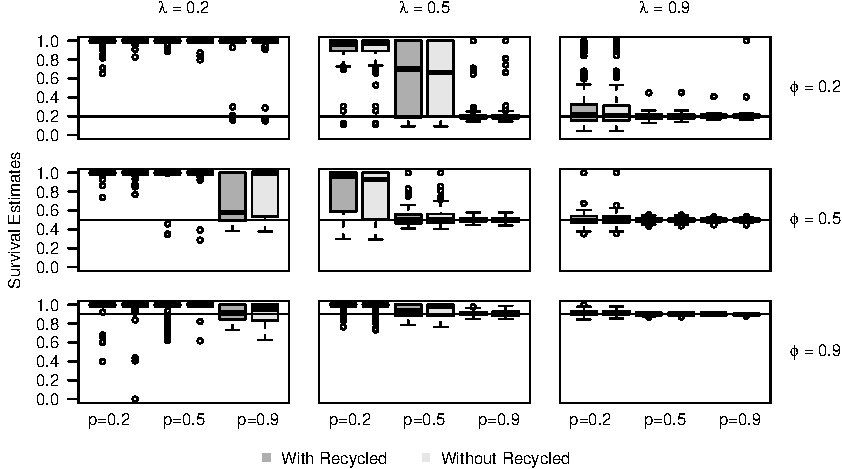
\includegraphics{Appendix_BW_files/figure-latex/figure1_survival_GJSTL1-1.pdf}

\textsc{Web Figure 1:} Boxplots of survival estimates (\(\hat{\phi}\))
of 100 simulated datasets analyzed with and without the effect of
recycled individuals for population size \(1000\) with \(T_2=1\) with 10
sample times for varying survival (\(\phi=0.2,0.5,0.9\)), capture
(\(p=0.2,0.5,0.9\)), and tag retention (\(\lambda=0.2,0.5,0.9\))
probabilities. The black line indicates the true value of \(\phi\) used
to simulate the data for each model.

\textsc{Web Table 1:} Standard Error (SE), Standard Deviation (SD), and
Root Mean Squared Error (RMSE) of survival estimates (\(\hat{\phi}\)) of
100 simulated datasets analyzed without (R') and with (R) the effect of
recycled individuals with population size \(N=1000\) with \(T_2=1\) with
10 sample times for varying tag retention (\(\lambda=0.2,0.5,0.9\)),
varying survival probabilities (\(\phi=0.2,0.5,0.9\)) and varying
capture probabilities (\(p=0.2,0.5,0.9\)).

\begin{table}[ht]
\centering
\begingroup\setlength{\tabcolsep}{12pt}
\scalebox{0.7}{
\begin{tabular}{rrrrrrrrr}
  \hline
$\phi$ & p & $\lambda$ & SE (R') & SE (R) & SD (R') & SD (R) & RMSE (R') & RMSE (R) \\ 
  \hline
0.9 & 0.9 & 0.9 & 0.0066 & 0.0064 & 0.0066 & 0.0064 & 0.0069 & 0.0066 \\ 
  0.9 & 0.9 & 0.5 & 0.0334 & 0.0241 & 0.0327 & 0.0243 & 0.0337 & 0.0249 \\ 
  0.9 & 0.9 & 0.2 & 0.0796 & 0.0620 & 0.0926 & 0.0792 & 0.0941 & 0.0797 \\ 
  0.9 & 0.5 & 0.9 & 0.0095 & 0.0093 & 0.0097 & 0.0093 & 0.0096 & 0.0093 \\ 
  0.9 & 0.5 & 0.5 & 0.0286 & 0.0332 & 0.0683 & 0.0622 & 0.0801 & 0.0691 \\ 
  0.9 & 0.5 & 0.2 & 0.0039 & 0.0336 & 0.0420 & 0.0939 & 0.1032 & 0.1107 \\ 
  0.9 & 0.2 & 0.9 & 0.0224 & 0.0224 & 0.0249 & 0.0274 & 0.0291 & 0.0305 \\ 
  0.9 & 0.2 & 0.5 & 0.0213 & 0.0180 & 0.0620 & 0.0483 & 0.0963 & 0.0944 \\ 
  0.9 & 0.2 & 0.2 & 0.0117 & 0.0150 & 0.0837 & 0.0929 & 0.1190 & 0.1214 \\ 
  0.5 & 0.9 & 0.9 & 0.0138 & 0.0137 & 0.0132 & 0.0129 & 0.0132 & 0.0129 \\ 
  0.5 & 0.9 & 0.5 & 0.0307 & 0.0277 & 0.0317 & 0.0299 & 0.0318 & 0.0298 \\ 
  0.5 & 0.9 & 0.2 & 0.0544 & 0.0699 & 0.2501 & 0.2416 & 0.3815 & 0.3098 \\ 
  0.5 & 0.5 & 0.9 & 0.0212 & 0.0211 & 0.0217 & 0.0218 & 0.0216 & 0.0217 \\ 
  0.5 & 0.5 & 0.5 & 0.0554 & 0.0511 & 0.0969 & 0.1099 & 0.1002 & 0.1130 \\ 
  0.5 & 0.5 & 0.2 & 0.0059 & 0.0100 & 0.0934 & 0.1059 & 0.4943 & 0.4928 \\ 
  0.5 & 0.2 & 0.9 & 0.0465 & 0.0465 & 0.0870 & 0.0871 & 0.0880 & 0.0875 \\ 
  0.5 & 0.2 & 0.5 & 0.0651 & 0.0630 & 0.2466 & 0.2362 & 0.3861 & 0.3940 \\ 
  0.5 & 0.2 & 0.2 & 0.0135 & 0.0076 & 0.0334 & 0.0303 & 0.4929 & 0.4955 \\ 
  0.2 & 0.9 & 0.9 & 0.0147 & 0.0147 & 0.0857 & 0.0257 & 0.0865 & 0.0260 \\ 
  0.2 & 0.9 & 0.5 & 0.0264 & 0.0254 & 0.1393 & 0.1262 & 0.1420 & 0.1280 \\ 
  0.2 & 0.9 & 0.2 & 0.0058 & 0.0071 & 0.1597 & 0.2061 & 0.7824 & 0.7709 \\ 
  0.2 & 0.5 & 0.9 & 0.0310 & 0.0308 & 0.0507 & 0.0448 & 0.0508 & 0.0446 \\ 
  0.2 & 0.5 & 0.5 & 0.0481 & 0.0500 & 0.3683 & 0.3729 & 0.5306 & 0.5476 \\ 
  0.2 & 0.5 & 0.2 & 0.0039 & 0.0042 & 0.0289 & 0.0154 & 0.7955 & 0.7976 \\ 
  0.2 & 0.2 & 0.9 & 0.0692 & 0.0701 & 0.2481 & 0.2485 & 0.2661 & 0.2682 \\ 
  0.2 & 0.2 & 0.5 & 0.0586 & 0.0677 & 0.1722 & 0.1681 & 0.7256 & 0.7278 \\ 
  0.2 & 0.2 & 0.2 & 0.0086 & 0.0213 & 0.0266 & 0.0563 & 0.7951 & 0.7848 \\ 
   \hline
\end{tabular}
}
\endgroup
\end{table}

\newpage 

\paragraph{N=100000, T=1}\label{n100000-t1}

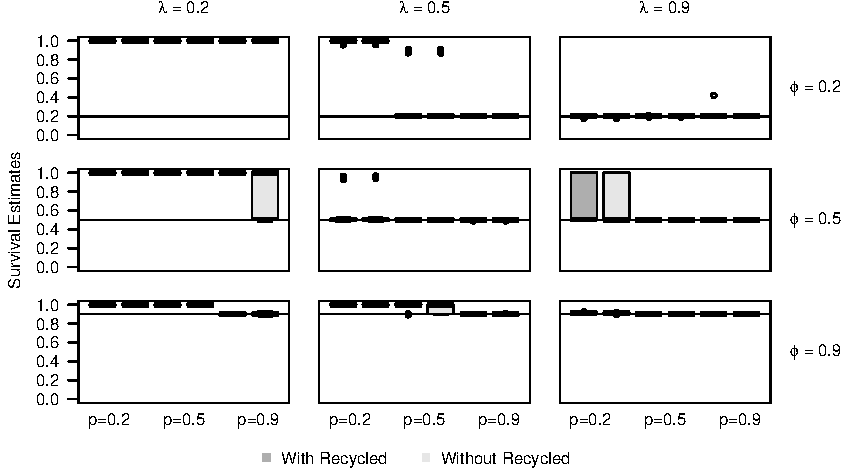
\includegraphics{Appendix_BW_files/figure-latex/figure2_survival_GJSTL2-1.pdf}

\textsc{Web Figure 2:} Boxplots of survival estimates (\(\hat{\phi}\))
of 100 simulated datasets analyzed with and without the effect of
recycled individuals for population size \(100000\) with \(T_2=1\) with
10 sample times for varying survival (\(\phi=0.2,0.5,0.9\)), capture
(\(p=0.2,0.5,0.9\)), and tag retention (\(\lambda=0.2,0.5,0.9\))
probabilities. The black line indicates the true value of \(\phi\) used
to simulate the data for each model.

\textsc{Web Table 2:} Standard Error (SE), Standard Deviation (SD), and
Root Mean Squared Error (RMSE) of survival estimates (\(\hat{\phi}\)) of
100 simulated datasets analyzed without (R') and with (R) the effect of
recycled individuals with population size \(N=100000\) with \(T_2=1\)
with 10 sample times for varying tag retention
(\(\lambda=0.2,0.5,0.9\)), varying survival probabilities
(\(\phi=0.2,0.5,0.9\)) and varying capture probabilities
(\(p=0.2,0.5,0.9\)).

\begin{table}[ht]
\centering
\begingroup\setlength{\tabcolsep}{12pt}
\scalebox{0.8}{
\begin{tabular}{rrrrrrrrr}
  \hline
$\phi$ & p & $\lambda$ & SE (R') & SE (R) & SD (R') & SD (R) & RMSE (R') & RMSE (R) \\ 
  \hline
0.9 & 0.9 & 0.9 & 0.0007 & 0.0006 & 0.0006 & 0.0006 & 0.0006 & 0.0006 \\ 
  0.9 & 0.9 & 0.5 & 0.0032 & 0.0024 & 0.0031 & 0.0023 & 0.0031 & 0.0024 \\ 
  0.9 & 0.9 & 0.2 & 0.0138 & 0.0083 & 0.0136 & 0.0088 & 0.0135 & 0.0087 \\ 
  0.9 & 0.5 & 0.9 & 0.0009 & 0.0009 & 0.0009 & 0.0009 & 0.0009 & 0.0009 \\ 
  0.9 & 0.5 & 0.5 & 0.0048 & 0.0039 & 0.0510 & 0.0342 & 0.0742 & 0.0933 \\ 
  0.9 & 0.5 & 0.2 & 0.0000 & 0.0000 & 0.0000 & 0.0000 & 0.1000 & 0.1000 \\ 
  0.9 & 0.2 & 0.9 & 0.0022 & 0.0022 & 0.0027 & 0.0025 & 0.0132 & 0.0144 \\ 
  0.9 & 0.2 & 0.5 & 0.0001 & 0.0000 & 0.0000 & 0.0000 & 0.1000 & 0.1000 \\ 
  0.9 & 0.2 & 0.2 & 0.0000 & 0.0000 & 0.0000 & 0.0000 & 0.1000 & 0.1000 \\ 
  0.5 & 0.9 & 0.9 & 0.0014 & 0.0014 & 0.0014 & 0.0014 & 0.0014 & 0.0014 \\ 
  0.5 & 0.9 & 0.5 & 0.0030 & 0.0028 & 0.0032 & 0.0028 & 0.0032 & 0.0028 \\ 
  0.5 & 0.9 & 0.2 & 0.0100 & 0.0000 & 0.2228 & 0.0000 & 0.4272 & 0.5000 \\ 
  0.5 & 0.5 & 0.9 & 0.0021 & 0.0021 & 0.0021 & 0.0021 & 0.0021 & 0.0021 \\ 
  0.5 & 0.5 & 0.5 & 0.0054 & 0.0051 & 0.0055 & 0.0056 & 0.0054 & 0.0056 \\ 
  0.5 & 0.5 & 0.2 & 0.0000 & 0.0000 & 0.0000 & 0.0000 & 0.5000 & 0.5000 \\ 
  0.5 & 0.2 & 0.9 & 0.0033 & 0.0028 & 0.2351 & 0.2479 & 0.2829 & 0.3202 \\ 
  0.5 & 0.2 & 0.5 & 0.0123 & 0.0120 & 0.1297 & 0.1157 & 0.1357 & 0.1197 \\ 
  0.5 & 0.2 & 0.2 & 0.0001 & 0.0001 & 0.0000 & 0.0000 & 0.5000 & 0.5000 \\ 
  0.2 & 0.9 & 0.9 & 0.0015 & 0.0015 & 0.0014 & 0.0311 & 0.0014 & 0.0312 \\ 
  0.2 & 0.9 & 0.5 & 0.0025 & 0.0024 & 0.0026 & 0.0025 & 0.0026 & 0.0026 \\ 
  0.2 & 0.9 & 0.2 & 0.0000 & 0.0000 & 0.0000 & 0.0000 & 0.8000 & 0.8000 \\ 
  0.2 & 0.5 & 0.9 & 0.0031 & 0.0031 & 0.0032 & 0.0032 & 0.0032 & 0.0032 \\ 
  0.2 & 0.5 & 0.5 & 0.0064 & 0.0065 & 0.2382 & 0.2703 & 0.2556 & 0.2988 \\ 
  0.2 & 0.5 & 0.2 & 0.0002 & 0.0001 & 0.0000 & 0.0000 & 0.8000 & 0.8000 \\ 
  0.2 & 0.2 & 0.9 & 0.0074 & 0.0074 & 0.0074 & 0.0074 & 0.0073 & 0.0073 \\ 
  0.2 & 0.2 & 0.5 & 0.0070 & 0.0065 & 0.0117 & 0.0109 & 0.7946 & 0.7953 \\ 
  0.2 & 0.2 & 0.2 & 0.0002 & 0.0002 & 0.0000 & 0.0000 & 0.8000 & 0.8000 \\ 
   \hline
\end{tabular}
}
\endgroup
\end{table}

\newpage

\paragraph{N=1000, T=0.5}\label{n1000-t0.5}

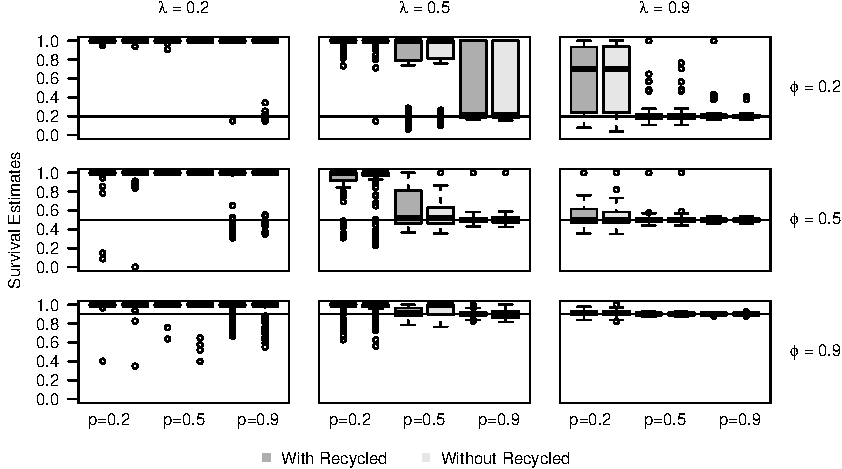
\includegraphics{Appendix_BW_files/figure-latex/figure3_survival_GJSTL4-1.pdf}

\textsc{Web Figure 3:} Boxplots of survival estimates (\(\hat{\phi}\))
of 100 simulated datasets analyzed with and without the effect of
recycled individuals for population size \(1000\) with \(T_2=0.5\) with
10 sample times for varying survival (\(\phi=0.2,0.5,0.9\)), capture
(\(p=0.2,0.5,0.9\)), and tag retention (\(\lambda=0.2,0.5,0.9\))
probabilities. The black line indicates the true value of \(\phi\) used
to simulate the data for each model.

\textsc{Web Table 3:} Standard Error (SE), Standard Deviation (SD), and
Root Mean Squared Error (RMSE) of survival estimates (\(\hat{\phi}\)) of
100 simulated datasets analyzed without (R') and with (R) the effect of
recycled individuals with population size \(N=1000\) with \(T_2=0.5\)
with 10 sample times for varying tag retention
(\(\lambda=0.2,0.5,0.9\)), varying survival probabilities
(\(\phi=0.2,0.5,0.9\)) and varying capture probabilities
(\(p=0.2,0.5,0.9\)).

\begin{table}[ht]
\centering
\begingroup\setlength{\tabcolsep}{12pt}
\scalebox{0.7}{
\begin{tabular}{rrrrrrrrr}
  \hline
$\phi$ & p & $\lambda$ & SE (R') & SE (R) & SD (R') & SD (R) & RMSE (R') & RMSE (R) \\ 
  \hline
0.9 & 0.9 & 0.9 & 0.0082 & 0.0077 & 0.0085 & 0.0080 & 0.0085 & 0.0081 \\ 
  0.9 & 0.9 & 0.5 & 0.0459 & 0.0319 & 0.0458 & 0.0311 & 0.0456 & 0.0312 \\ 
  0.9 & 0.9 & 0.2 & 0.0294 & 0.0389 & 0.1177 & 0.0939 & 0.1262 & 0.1069 \\ 
  0.9 & 0.5 & 0.9 & 0.0115 & 0.0111 & 0.0109 & 0.0110 & 0.0109 & 0.0110 \\ 
  0.9 & 0.5 & 0.5 & 0.0257 & 0.0462 & 0.0725 & 0.0589 & 0.0888 & 0.0611 \\ 
  0.9 & 0.5 & 0.2 & 0.0063 & 0.0044 & 0.0932 & 0.0434 & 0.1234 & 0.1034 \\ 
  0.9 & 0.2 & 0.9 & 0.0256 & 0.0256 & 0.0312 & 0.0307 & 0.0332 & 0.0335 \\ 
  0.9 & 0.2 & 0.5 & 0.0311 & 0.0233 & 0.0916 & 0.0935 & 0.1063 & 0.1106 \\ 
  0.9 & 0.2 & 0.2 & 0.0066 & 0.0041 & 0.0676 & 0.0599 & 0.1128 & 0.1110 \\ 
  0.5 & 0.9 & 0.9 & 0.0151 & 0.0148 & 0.0164 & 0.0160 & 0.0164 & 0.0160 \\ 
  0.5 & 0.9 & 0.5 & 0.0410 & 0.0361 & 0.0646 & 0.0615 & 0.0645 & 0.0614 \\ 
  0.5 & 0.9 & 0.2 & 0.0109 & 0.0203 & 0.1496 & 0.2041 & 0.4801 & 0.4628 \\ 
  0.5 & 0.5 & 0.9 & 0.0215 & 0.0215 & 0.1396 & 0.1227 & 0.1437 & 0.1249 \\ 
  0.5 & 0.5 & 0.5 & 0.0693 & 0.0534 & 0.1787 & 0.2249 & 0.1971 & 0.2548 \\ 
  0.5 & 0.5 & 0.2 & 0.0004 & 0.0003 & 0.0000 & 0.0000 & 0.5000 & 0.5000 \\ 
  0.5 & 0.2 & 0.9 & 0.0468 & 0.0459 & 0.1756 & 0.1849 & 0.1891 & 0.2002 \\ 
  0.5 & 0.2 & 0.5 & 0.0390 & 0.0376 & 0.2110 & 0.1979 & 0.4543 & 0.4481 \\ 
  0.5 & 0.2 & 0.2 & 0.0094 & 0.0104 & 0.0279 & 0.1262 & 0.4945 & 0.4942 \\ 
  0.2 & 0.9 & 0.9 & 0.0158 & 0.0154 & 0.0372 & 0.1430 & 0.0373 & 0.1453 \\ 
  0.2 & 0.9 & 0.5 & 0.0303 & 0.0251 & 0.3840 & 0.3924 & 0.4876 & 0.5078 \\ 
  0.2 & 0.9 & 0.2 & 0.0073 & 0.0008 & 0.1702 & 0.0851 & 0.7799 & 0.7960 \\ 
  0.2 & 0.5 & 0.9 & 0.0326 & 0.0325 & 0.0976 & 0.1181 & 0.0982 & 0.1197 \\ 
  0.2 & 0.5 & 0.5 & 0.0405 & 0.0348 & 0.3305 & 0.3247 & 0.6892 & 0.6895 \\ 
  0.2 & 0.5 & 0.2 & 0.0008 & 0.0027 & 0.0000 & 0.0097 & 0.8000 & 0.7988 \\ 
  0.2 & 0.2 & 0.9 & 0.0644 & 0.0661 & 0.3416 & 0.3369 & 0.5360 & 0.5223 \\ 
  0.2 & 0.2 & 0.5 & 0.0273 & 0.0278 & 0.0952 & 0.0455 & 0.7811 & 0.7839 \\ 
  0.2 & 0.2 & 0.2 & 0.0009 & 0.0028 & 0.0061 & 0.0057 & 0.7994 & 0.7991 \\ 
   \hline
\end{tabular}
}
\endgroup
\end{table}

\newpage

\paragraph{N=100000, T=0.5}\label{n100000-t0.5}

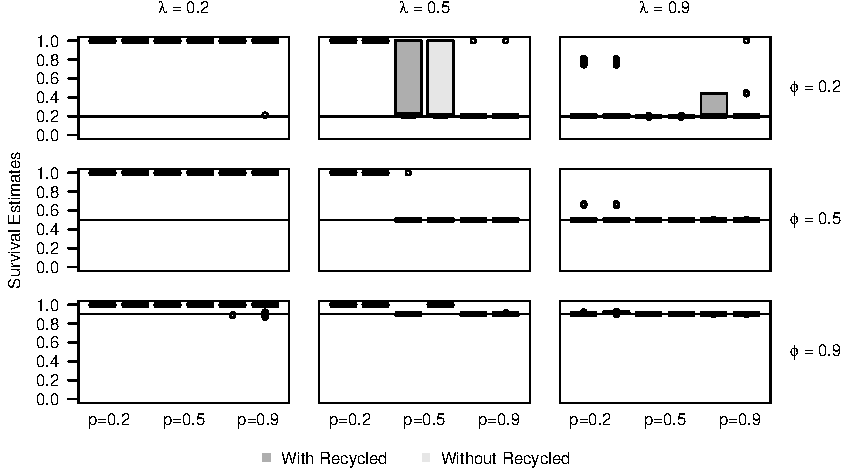
\includegraphics{Appendix_BW_files/figure-latex/figure4_survival_GJSTL3-1.pdf}

\textsc{Web Figure 4:} Boxplots of survival estimates (\(\hat{\phi}\))
of 100 simulated datasets analyzed with and without the effect of
recycled individuals for population size \(100000\) with \(T_2=0.5\)
with 10 sample times for varying survival (\(\phi=0.2,0.5,0.9\)),
capture (\(p=0.2,0.5,0.9\)), and tag retention (\(\lambda=0.2,0.5,0.9\))
probabilities. The black line indicates the true value of \(\phi\) used
to simulate the data for each model.

\textsc{Web Table 4:} Standard Error (SE), Standard Deviation (SD), and
Root Mean Squared Error (RMSE) of survival estimates (\(\hat{\phi}\)) of
100 simulated datasets analyzed without (R') and with (R) the effect of
recycled individuals with population size \(N=100000\) with \(T_2=0.5\)
with 10 sample times for varying tag retention
(\(\lambda=0.2,0.5,0.9\)), varying survival probabilities
(\(\phi=0.2,0.5,0.9\)) and varying capture probabilities
(\(p=0.2,0.5,0.9\)).

\begin{table}[ht]
\centering
\begingroup\setlength{\tabcolsep}{12pt}
\scalebox{0.7}{
\begin{tabular}{rrrrrrrrr}
  \hline
$\phi$ & p & $\lambda$ & SE (R') & SE (R) & SD (R') & SD (R) & RMSE (R') & RMSE (R) \\ 
  \hline
0.9 & 0.9 & 0.9 & 0.0008 & 0.0008 & 0.0009 & 0.0009 & 0.0009 & 0.0009 \\ 
  0.9 & 0.9 & 0.5 & 0.0045 & 0.0032 & 0.0052 & 0.0033 & 0.0052 & 0.0034 \\ 
  0.9 & 0.9 & 0.2 & 0.0179 & 0.0073 & 0.0343 & 0.0155 & 0.0932 & 0.0988 \\ 
  0.9 & 0.5 & 0.9 & 0.0012 & 0.0011 & 0.0010 & 0.0010 & 0.0010 & 0.0010 \\ 
  0.9 & 0.5 & 0.5 & 0.0000 & 0.0055 & 0.0000 & 0.0052 & 0.1000 & 0.0052 \\ 
  0.9 & 0.5 & 0.2 & 0.0000 & 0.0000 & 0.0000 & 0.0001 & 0.1000 & 0.0999 \\ 
  0.9 & 0.2 & 0.9 & 0.0026 & 0.0026 & 0.0055 & 0.0060 & 0.0165 & 0.0064 \\ 
  0.9 & 0.2 & 0.5 & 0.0000 & 0.0000 & 0.0000 & 0.0000 & 0.1000 & 0.1000 \\ 
  0.9 & 0.2 & 0.2 & 0.0000 & 0.0000 & 0.0000 & 0.0000 & 0.1000 & 0.1000 \\ 
  0.5 & 0.9 & 0.9 & 0.0015 & 0.0015 & 0.0014 & 0.0014 & 0.0014 & 0.0014 \\ 
  0.5 & 0.9 & 0.5 & 0.0041 & 0.0036 & 0.0041 & 0.0037 & 0.0041 & 0.0037 \\ 
  0.5 & 0.9 & 0.2 & 0.0000 & 0.0000 & 0.0000 & 0.0000 & 0.5000 & 0.5000 \\ 
  0.5 & 0.5 & 0.9 & 0.0023 & 0.0023 & 0.0020 & 0.0020 & 0.0020 & 0.0020 \\ 
  0.5 & 0.5 & 0.5 & 0.0068 & 0.0064 & 0.0068 & 0.0510 & 0.0068 & 0.0509 \\ 
  0.5 & 0.5 & 0.2 & 0.0000 & 0.0000 & 0.0000 & 0.0000 & 0.5000 & 0.5000 \\ 
  0.5 & 0.2 & 0.9 & 0.0052 & 0.0051 & 0.0566 & 0.0442 & 0.0612 & 0.0463 \\ 
  0.5 & 0.2 & 0.5 & 0.0000 & 0.0000 & 0.0000 & 0.0000 & 0.5000 & 0.5000 \\ 
  0.5 & 0.2 & 0.2 & 0.0002 & 0.0002 & 0.0000 & 0.0000 & 0.5000 & 0.5000 \\ 
  0.2 & 0.9 & 0.9 & 0.0018 & 0.0020 & 0.1240 & 0.1154 & 0.1367 & 0.1414 \\ 
  0.2 & 0.9 & 0.5 & 0.0031 & 0.0029 & 0.2704 & 0.2871 & 0.2885 & 0.3098 \\ 
  0.2 & 0.9 & 0.2 & 0.0005 & 0.0000 & 0.0788 & 0.0000 & 0.7960 & 0.8000 \\ 
  0.2 & 0.5 & 0.9 & 0.0033 & 0.0033 & 0.0032 & 0.0032 & 0.0033 & 0.0032 \\ 
  0.2 & 0.5 & 0.5 & 0.0064 & 0.0063 & 0.3971 & 0.4020 & 0.5184 & 0.5484 \\ 
  0.2 & 0.5 & 0.2 & 0.0001 & 0.0001 & 0.0000 & 0.0000 & 0.8000 & 0.8000 \\ 
  0.2 & 0.2 & 0.9 & 0.0085 & 0.0086 & 0.2210 & 0.2344 & 0.2438 & 0.2634 \\ 
  0.2 & 0.2 & 0.5 & 0.0007 & 0.0007 & 0.0001 & 0.0001 & 0.7999 & 0.7999 \\ 
  0.2 & 0.2 & 0.2 & 0.0003 & 0.0003 & 0.0000 & 0.0000 & 0.8000 & 0.8000 \\ 
   \hline
\end{tabular}
}
\endgroup
\end{table}

\newpage

\paragraph{N=1000, T=1, t=5}\label{n1000-t1-t5}

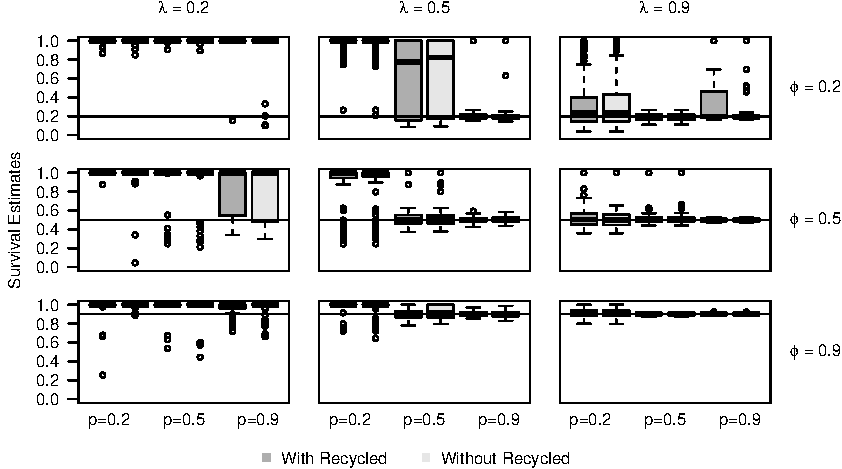
\includegraphics{Appendix_BW_files/figure-latex/figure5_survival_GJSTL5-1.pdf}

\textsc{Web Figure 5:} Boxplots of survival estimates (\(\hat{\phi}\))
of 100 simulated datasets analyzed with and without the effect of
recycled individuals for population size \(1000\) with \(T_2=1\) with 5
sample times for varying survival (\(\phi=0.2,0.5,0.9\)), capture
(\(p=0.2,0.5,0.9\)), and tag retention (\(\lambda=0.2,0.5,0.9\))
probabilities. The black line indicates the true value of \(\phi\) used
to simulate the data for each model.

\paragraph{N=1000, T=1, t=7}\label{n1000-t1-t7}

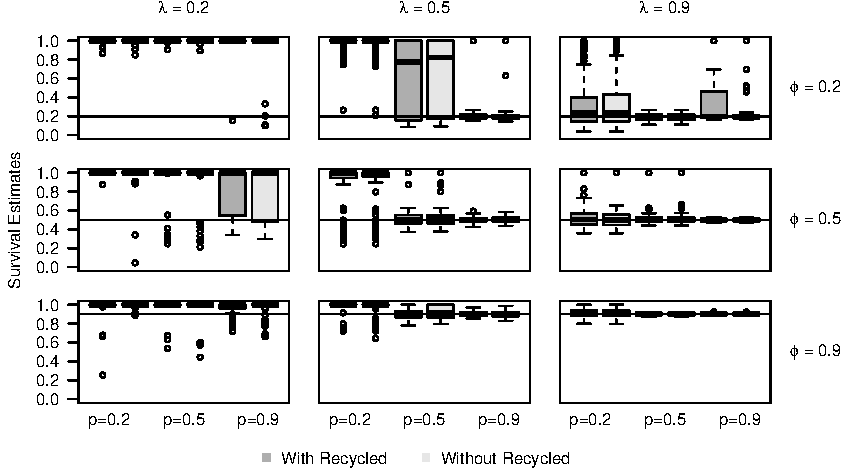
\includegraphics{Appendix_BW_files/figure-latex/figure6_survival_GJSTL6-1.pdf}

\textsc{Web Figure 6:} Boxplots of survival estimates (\(\hat{\phi}\))
of 100 simulated datasets analyzed with and without the effect of
recycled individuals for population size \(1000\) with \(T_2=1\) with 7
sample times for varying survival (\(\phi=0.2,0.5,0.9\)), capture
(\(p=0.2,0.5,0.9\)), and tag retention (\(\lambda=0.2,0.5,0.9\))
probabilities. The black line indicates the true value of \(\phi\) used
to simulate the data for each model.

\newpage

\subsection{Capture Estimates}\label{capture-estimates}

\paragraph{N=1000, T=1}\label{n1000-t1-1}

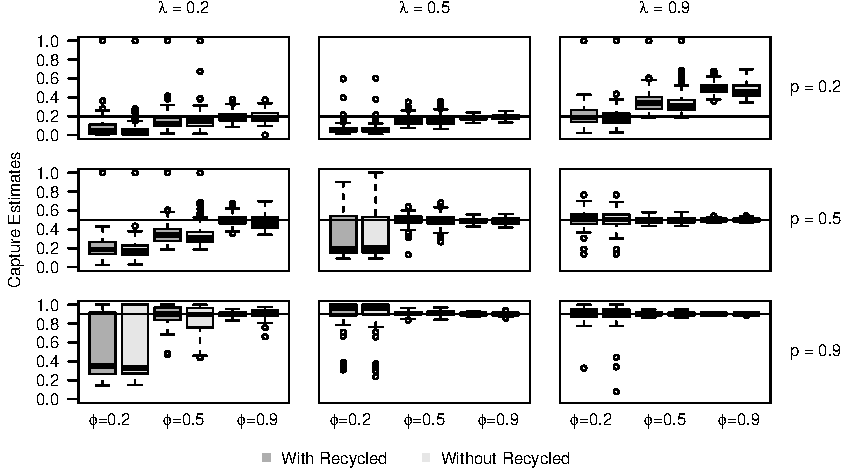
\includegraphics{Appendix_BW_files/figure-latex/figure7_capture_GJSTL1-1.pdf}

\textsc{Web Figure 7:} Boxplots of capture estimates (\(\hat{p}\)) of
100 simulated datasets analyzed with and without the effect of recycled
individuals for population size \(1000\) with \(T_2=1\) with 10 sample times for varying survival (\(\phi=0.2,0.5,0.9\)), capture
(\(p=0.2,0.5,0.9\)), and tag retention (\(\lambda=0.2,0.5,0.9\))
probabilities. The black line indicates the true value of \(p\) used to
simulate the data for each model.

\textsc{Web Table 5:} Standard Error (SE), Standard Deviation (SD), and
Root Mean Squared Error (RMSE) of capture estimates (\(\hat{p}\))of 100
simulated datasets analyzed without (R') and with (R) the effect of
recycled individuals with population size \(N=1000\) with \(T_2=1\) with
10 sample times for varying tag retention (\(\lambda=0.2,0.5,0.9\)),
varying survival probabilities (\(\phi=0.2,0.5,0.9\)) and varying
capture probabilities (\(p=0.2,0.5,0.9\)).

\begin{table}[ht]
\centering
\begingroup\setlength{\tabcolsep}{12pt}
\scalebox{0.7}{
\begin{tabular}{rrrrrrrrr}
  \hline
$\phi$ & p & $\lambda$ & SE (R') & SE (R) & SD (R') & SD (R) & RMSE (R') & RMSE (R) \\ 
  \hline
0.9 & 0.9 & 0.9 & 0.0066 & 0.0065 & 0.0063 & 0.0060 & 0.0063 & 0.0060 \\ 
  0.9 & 0.9 & 0.5 & 0.0139 & 0.0106 & 0.0147 & 0.0116 & 0.0146 & 0.0116 \\ 
  0.9 & 0.9 & 0.2 & 0.0374 & 0.0245 & 0.0484 & 0.0251 & 0.0484 & 0.0251 \\ 
  0.9 & 0.5 & 0.9 & 0.0131 & 0.0129 & 0.0151 & 0.0148 & 0.0150 & 0.0147 \\ 
  0.9 & 0.5 & 0.5 & 0.0251 & 0.0213 & 0.0343 & 0.0269 & 0.0365 & 0.0283 \\ 
  0.9 & 0.5 & 0.2 & 0.0574 & 0.0470 & 0.0746 & 0.0590 & 0.0793 & 0.0587 \\ 
  0.9 & 0.2 & 0.9 & 0.0147 & 0.0147 & 0.0167 & 0.0178 & 0.0180 & 0.0186 \\ 
  0.9 & 0.2 & 0.5 & 0.0227 & 0.0203 & 0.0250 & 0.0225 & 0.0267 & 0.0260 \\ 
  0.9 & 0.2 & 0.2 & 0.0530 & 0.0470 & 0.0557 & 0.0514 & 0.0555 & 0.0515 \\ 
  0.5 & 0.9 & 0.9 & 0.0167 & 0.0166 & 0.0172 & 0.0172 & 0.0174 & 0.0173 \\ 
  0.5 & 0.9 & 0.5 & 0.0275 & 0.0251 & 0.0262 & 0.0256 & 0.0270 & 0.0264 \\ 
  0.5 & 0.9 & 0.2 & 0.0592 & 0.0570 & 0.1815 & 0.1119 & 0.1974 & 0.1128 \\ 
  0.5 & 0.5 & 0.9 & 0.0323 & 0.0322 & 0.0331 & 0.0329 & 0.0330 & 0.0328 \\ 
  0.5 & 0.5 & 0.5 & 0.0526 & 0.0498 & 0.0665 & 0.0680 & 0.0662 & 0.0678 \\ 
  0.5 & 0.5 & 0.2 & 0.0717 & 0.0696 & 0.1207 & 0.1175 & 0.1979 & 0.1852 \\ 
  0.5 & 0.2 & 0.9 & 0.0339 & 0.0342 & 0.0462 & 0.0457 & 0.0459 & 0.0455 \\ 
  0.5 & 0.2 & 0.5 & 0.0385 & 0.0357 & 0.0631 & 0.0562 & 0.0730 & 0.0709 \\ 
  0.5 & 0.2 & 0.2 & 0.0621 & 0.0536 & 0.1698 & 0.1628 & 0.1704 & 0.1650 \\ 
  0.2 & 0.9 & 0.9 & 0.0426 & 0.0428 & 0.1209 & 0.0769 & 0.1205 & 0.0768 \\ 
  0.2 & 0.9 & 0.5 & 0.0467 & 0.0489 & 0.1644 & 0.1473 & 0.1636 & 0.1466 \\ 
  0.2 & 0.9 & 0.2 & 0.0673 & 0.0785 & 0.3190 & 0.3079 & 0.5023 & 0.4954 \\ 
  0.2 & 0.5 & 0.9 & 0.0916 & 0.0926 & 0.0997 & 0.0952 & 0.0992 & 0.0951 \\ 
  0.2 & 0.5 & 0.5 & 0.0795 & 0.0789 & 0.2462 & 0.2420 & 0.2888 & 0.2873 \\ 
  0.2 & 0.5 & 0.2 & 0.0626 & 0.0655 & 0.2080 & 0.2367 & 0.3364 & 0.3405 \\ 
  0.2 & 0.2 & 0.9 & 0.0912 & 0.0895 & 0.2011 & 0.2017 & 0.2021 & 0.2023 \\ 
  0.2 & 0.2 & 0.5 & 0.0310 & 0.0318 & 0.0714 & 0.0716 & 0.1487 & 0.1480 \\ 
  0.2 & 0.2 & 0.2 & 0.0266 & 0.0384 & 0.1145 & 0.1184 & 0.1792 & 0.1698 \\ 
   \hline
\end{tabular}
}
\endgroup
\end{table}

\newpage

\paragraph{N=100000, T=1}\label{n100000-t1-1}

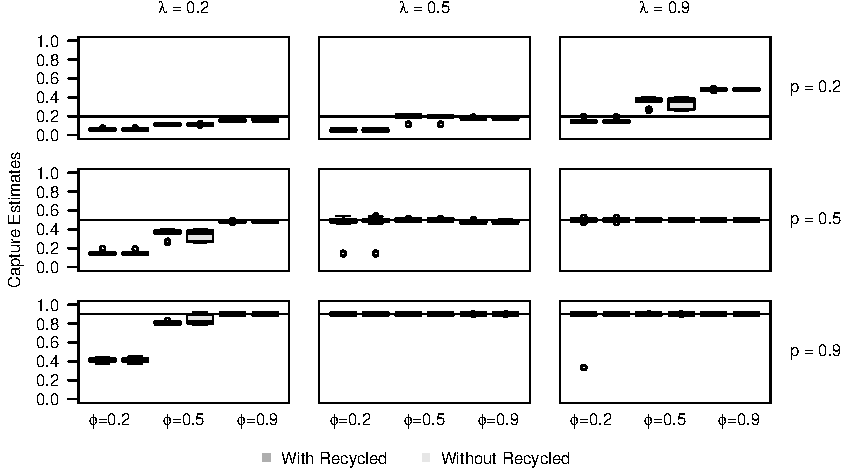
\includegraphics{Appendix_BW_files/figure-latex/8_capture_GJSTL2-1.pdf}

\textsc{Web Figure 8:} Boxplots of capture estimates (\(\hat{p}\)) of
100 simulated datasets analyzed with and without the effect of recycled
individuals for population size \(100000\) with \(T_2=1\) with 10 sample times for varying survival (\(\phi=0.2,0.5,0.9\)), capture
(\(p=0.2,0.5,0.9\)), and tag retention (\(\lambda=0.2,0.5,0.9\))
probabilities. The black line indicates the true value of \(p\) used to
simulate the data for each model.

\textsc{Web Table 6:} Standard Error (SE), Standard Deviation (SD), and
Root Mean Squared Error (RMSE) of capture estimates (\(\hat{p}\)) of 100
simulated datasets analyzed without (R') and with (R) the effect of
recycled individuals with population size \(N=100000\) with \(T_2=1\)
with 10 sample times for varying tag retention
(\(\lambda=0.2,0.5,0.9\)), varying survival probabilities
(\(\phi=0.2,0.5,0.9\)) and varying capture probabilities
(\(p=0.2,0.5,0.9\)).

\begin{table}[ht]
\centering
\begingroup\setlength{\tabcolsep}{12pt}
\scalebox{0.7}{
\begin{tabular}{rrrrrrrrr}
  \hline
$\phi$ & p & $\lambda$ & SE (R') & SE (R) & SD (R') & SD (R) & RMSE (R') & RMSE (R) \\ 
  \hline
0.9 & 0.9 & 0.9 & 0.0007 & 0.0006 & 0.0007 & 0.0007 & 0.0007 & 0.0007 \\ 
  0.9 & 0.9 & 0.5 & 0.0014 & 0.0011 & 0.0013 & 0.0011 & 0.0013 & 0.0011 \\ 
  0.9 & 0.9 & 0.2 & 0.0039 & 0.0025 & 0.0035 & 0.0023 & 0.0035 & 0.0023 \\ 
  0.9 & 0.5 & 0.9 & 0.0013 & 0.0013 & 0.0012 & 0.0012 & 0.0012 & 0.0012 \\ 
  0.9 & 0.5 & 0.5 & 0.0025 & 0.0020 & 0.0125 & 0.0090 & 0.0176 & 0.0228 \\ 
  0.9 & 0.5 & 0.2 & 0.0062 & 0.0045 & 0.0062 & 0.0045 & 0.0171 & 0.0172 \\ 
  0.9 & 0.2 & 0.9 & 0.0015 & 0.0015 & 0.0018 & 0.0016 & 0.0084 & 0.0091 \\ 
  0.9 & 0.2 & 0.5 & 0.0021 & 0.0020 & 0.0033 & 0.0020 & 0.0188 & 0.0147 \\ 
  0.9 & 0.2 & 0.2 & 0.0041 & 0.0032 & 0.0038 & 0.0028 & 0.0361 & 0.0441 \\ 
  0.5 & 0.9 & 0.9 & 0.0017 & 0.0017 & 0.0017 & 0.0017 & 0.0016 & 0.0017 \\ 
  0.5 & 0.9 & 0.5 & 0.0029 & 0.0026 & 0.0029 & 0.0027 & 0.0028 & 0.0027 \\ 
  0.5 & 0.9 & 0.2 & 0.0098 & 0.0089 & 0.0426 & 0.0084 & 0.0782 & 0.0925 \\ 
  0.5 & 0.5 & 0.9 & 0.0032 & 0.0032 & 0.0033 & 0.0033 & 0.0033 & 0.0033 \\ 
  0.5 & 0.5 & 0.5 & 0.0054 & 0.0051 & 0.0059 & 0.0057 & 0.0059 & 0.0057 \\ 
  0.5 & 0.5 & 0.2 & 0.0075 & 0.0074 & 0.0539 & 0.0433 & 0.1715 & 0.1502 \\ 
  0.5 & 0.2 & 0.9 & 0.0025 & 0.0022 & 0.0739 & 0.0781 & 0.0892 & 0.1011 \\ 
  0.5 & 0.2 & 0.5 & 0.0053 & 0.0052 & 0.0249 & 0.0220 & 0.0260 & 0.0228 \\ 
  0.5 & 0.2 & 0.2 & 0.0045 & 0.0043 & 0.0038 & 0.0035 & 0.0863 & 0.0871 \\ 
  0.2 & 0.9 & 0.9 & 0.0050 & 0.0050 & 0.0043 & 0.0796 & 0.0043 & 0.0801 \\ 
  0.2 & 0.9 & 0.5 & 0.0077 & 0.0075 & 0.0078 & 0.0078 & 0.0078 & 0.0077 \\ 
  0.2 & 0.9 & 0.2 & 0.0160 & 0.0151 & 0.0149 & 0.0136 & 0.4861 & 0.4862 \\ 
  0.2 & 0.5 & 0.9 & 0.0092 & 0.0092 & 0.0098 & 0.0098 & 0.0097 & 0.0097 \\ 
  0.2 & 0.5 & 0.5 & 0.0125 & 0.0118 & 0.1248 & 0.1411 & 0.1340 & 0.1561 \\ 
  0.2 & 0.5 & 0.2 & 0.0053 & 0.0051 & 0.0067 & 0.0068 & 0.3540 & 0.3544 \\ 
  0.2 & 0.2 & 0.9 & 0.0093 & 0.0092 & 0.0092 & 0.0092 & 0.0092 & 0.0092 \\ 
  0.2 & 0.2 & 0.5 & 0.0021 & 0.0021 & 0.0020 & 0.0019 & 0.1478 & 0.1479 \\ 
  0.2 & 0.2 & 0.2 & 0.0046 & 0.0045 & 0.0040 & 0.0040 & 0.1402 & 0.1403 \\ 
   \hline
\end{tabular}
}
\endgroup
\end{table}

\newpage

\paragraph{N=1000, T=0.5}\label{n1000-t0.5-1}

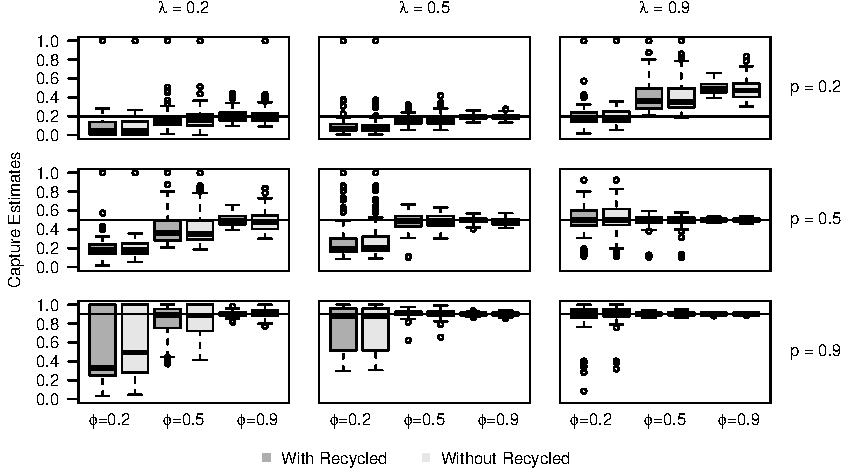
\includegraphics{Appendix_BW_files/figure-latex/figure9_capture_GJSTL4-1.pdf}

\textsc{Web Figure 9:} Boxplots of capture estimates (\(\hat{p}\)) of
100 simulated datasets analyzed with and without the effect of recycled
individuals for population size \(1000\) with \(T_2=0.5\) with 10 sample times for varying survival (\(\phi=0.2,0.5,0.9\)), capture
(\(p=0.2,0.5,0.9\)), and tag retention (\(\lambda=0.2,0.5,0.9\))
probabilities. The black line indicates the true value of \(p\) used to
simulate the data for each model.

\textsc{Web Table 7:} Standard Error (SE), Standard Deviation (SD), and
Root Mean Squared Error (RMSE) of capture estimates (\(\hat{p}\)) of 100
simulated datasets analyzed without (R') and with (R) the effect of
recycled individuals with population size \(N=1000\) with \(T_2=0.5\)
with 10 sample times for varying tag retention
(\(\lambda=0.2,0.5,0.9\)), varying survival probabilities
(\(\phi=0.2,0.5,0.9\)) and varying capture probabilities
(\(p=0.2,0.5,0.9\)).

\begin{table}[ht]
\centering
\begingroup\setlength{\tabcolsep}{12pt}
\scalebox{0.7}{
\begin{tabular}{rrrrrrrrr}
  \hline
$\phi$ & p & $\lambda$ & SE (R') & SE (R) & SD (R') & SD (R) & RMSE (R') & RMSE (R) \\ 
  \hline
0.9 & 0.9 & 0.9 & 0.0070 & 0.0066 & 0.0065 & 0.0063 & 0.0066 & 0.0063 \\ 
  0.9 & 0.9 & 0.5 & 0.0159 & 0.0115 & 0.0171 & 0.0118 & 0.0170 & 0.0118 \\ 
  0.9 & 0.9 & 0.2 & 0.0412 & 0.0269 & 0.0432 & 0.0272 & 0.0438 & 0.0271 \\ 
  0.9 & 0.5 & 0.9 & 0.0139 & 0.0134 & 0.0151 & 0.0140 & 0.0150 & 0.0140 \\ 
  0.9 & 0.5 & 0.5 & 0.0279 & 0.0239 & 0.0363 & 0.0290 & 0.0408 & 0.0291 \\ 
  0.9 & 0.5 & 0.2 & 0.0688 & 0.0549 & 0.1051 & 0.0602 & 0.1064 & 0.0599 \\ 
  0.9 & 0.2 & 0.9 & 0.0156 & 0.0152 & 0.0179 & 0.0170 & 0.0181 & 0.0175 \\ 
  0.9 & 0.2 & 0.5 & 0.0276 & 0.0247 & 0.0280 & 0.0244 & 0.0287 & 0.0256 \\ 
  0.9 & 0.2 & 0.2 & 0.0674 & 0.0622 & 0.1086 & 0.0699 & 0.1091 & 0.0696 \\ 
  0.5 & 0.9 & 0.9 & 0.0176 & 0.0173 & 0.0183 & 0.0178 & 0.0184 & 0.0179 \\ 
  0.5 & 0.9 & 0.5 & 0.0311 & 0.0277 & 0.0407 & 0.0397 & 0.0407 & 0.0398 \\ 
  0.5 & 0.9 & 0.2 & 0.0638 & 0.0612 & 0.2004 & 0.1960 & 0.2177 & 0.2129 \\ 
  0.5 & 0.5 & 0.9 & 0.0320 & 0.0321 & 0.1063 & 0.1001 & 0.1092 & 0.1015 \\ 
  0.5 & 0.5 & 0.5 & 0.0574 & 0.0520 & 0.0813 & 0.1080 & 0.0826 & 0.1120 \\ 
  0.5 & 0.5 & 0.2 & 0.1038 & 0.0960 & 0.1778 & 0.1638 & 0.1954 & 0.1866 \\ 
  0.5 & 0.2 & 0.9 & 0.0324 & 0.0318 & 0.0592 & 0.0613 & 0.0618 & 0.0646 \\ 
  0.5 & 0.2 & 0.5 & 0.0432 & 0.0399 & 0.0640 & 0.0555 & 0.0744 & 0.0710 \\ 
  0.5 & 0.2 & 0.2 & 0.0811 & 0.0812 & 0.2551 & 0.2047 & 0.2573 & 0.2037 \\ 
  0.2 & 0.9 & 0.9 & 0.0444 & 0.0437 & 0.1088 & 0.1639 & 0.1083 & 0.1654 \\ 
  0.2 & 0.9 & 0.5 & 0.0733 & 0.0723 & 0.2443 & 0.2453 & 0.2780 & 0.2848 \\ 
  0.2 & 0.9 & 0.2 & 0.0924 & 0.0772 & 0.3353 & 0.3400 & 0.4540 & 0.5007 \\ 
  0.2 & 0.5 & 0.9 & 0.0952 & 0.0935 & 0.1384 & 0.1450 & 0.1390 & 0.1445 \\ 
  0.2 & 0.5 & 0.5 & 0.0725 & 0.0707 & 0.1847 & 0.1933 & 0.2873 & 0.2928 \\ 
  0.2 & 0.5 & 0.2 & 0.0641 & 0.0659 & 0.2176 & 0.2122 & 0.3340 & 0.3404 \\ 
  0.2 & 0.2 & 0.9 & 0.0502 & 0.0511 & 0.1418 & 0.1057 & 0.1607 & 0.1355 \\ 
  0.2 & 0.2 & 0.5 & 0.0496 & 0.0484 & 0.1133 & 0.1435 & 0.1544 & 0.1723 \\ 
  0.2 & 0.2 & 0.2 & 0.0437 & 0.0381 & 0.2166 & 0.2775 & 0.2291 & 0.2801 \\ 
   \hline
\end{tabular}
}
\endgroup
\end{table}

\newpage

\paragraph{N=100000, T=0.5}\label{n100000-t0.5-1}

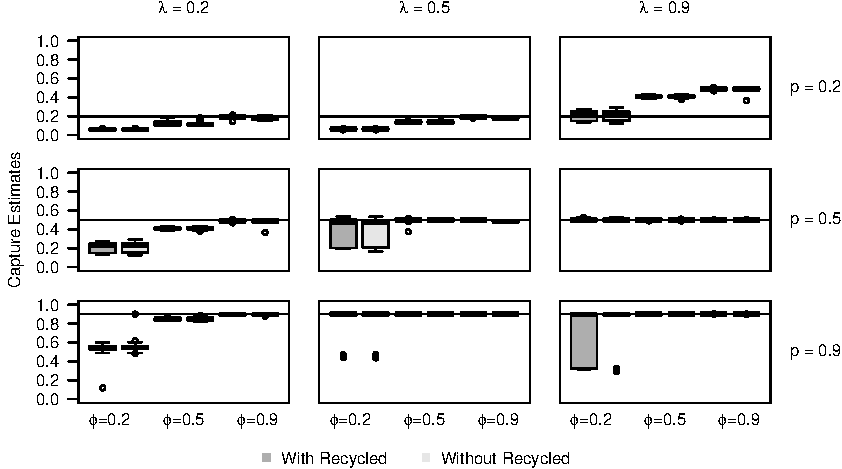
\includegraphics{Appendix_BW_files/figure-latex/figure10_capture_GJSTL3-1.pdf}

\textsc{Web Figure 10:} Boxplots of capture estimates (\(\hat{p}\)) of
100 simulated datasets analyzed with and without the effect of recycled
individuals for population size \(100000\) with \(T_2=0.5\) with 10 sample times for varying survival (\(\phi=0.2,0.5,0.9\)), capture
(\(p=0.2,0.5,0.9\)), and tag retention (\(\lambda=0.2,0.5,0.9\))
probabilities. The black line indicates the true value of \(p\) used to
simulate the data for each model.

\textsc{Web Table 8:} Standard Error (SE), Standard Deviation (SD), and
Root Mean Squared Error (RMSE) of capture estimates (\(\hat{p}\)) of 100
simulated datasets analyzed without (R') and with (R) the effect of
recycled individuals with population size \(N=100000\) with \(T_2=0.5\)
with 10 sample times for varying tag retention
(\(\lambda=0.2,0.5,0.9\)), varying survival probabilities
(\(\phi=0.2,0.5,0.9\)) and varying capture probabilities
(\(p=0.2,0.5,0.9\)).

\begin{table}[ht]
\centering
\begingroup\setlength{\tabcolsep}{12pt}
\scalebox{0.7}{
\begin{tabular}{rrrrrrrrr}
  \hline
$\phi$ & p & $\lambda$ & SE (R') & SE (R) & SD (R') & SD (R) & RMSE (R') & RMSE (R) \\ 
  \hline
0.9 & 0.9 & 0.9 & 0.0007 & 0.0007 & 0.0007 & 0.0007 & 0.0007 & 0.0007 \\ 
  0.9 & 0.9 & 0.5 & 0.0016 & 0.0011 & 0.0016 & 0.0011 & 0.0016 & 0.0011 \\ 
  0.9 & 0.9 & 0.2 & 0.0046 & 0.0028 & 0.0048 & 0.0032 & 0.0068 & 0.0058 \\ 
  0.9 & 0.5 & 0.9 & 0.0014 & 0.0013 & 0.0013 & 0.0013 & 0.0013 & 0.0013 \\ 
  0.9 & 0.5 & 0.5 & 0.0028 & 0.0024 & 0.0028 & 0.0024 & 0.0161 & 0.0024 \\ 
  0.9 & 0.5 & 0.2 & 0.0074 & 0.0053 & 0.0141 & 0.0052 & 0.0193 & 0.0131 \\ 
  0.9 & 0.2 & 0.9 & 0.0015 & 0.0016 & 0.0032 & 0.0033 & 0.0092 & 0.0035 \\ 
  0.9 & 0.2 & 0.5 & 0.0025 & 0.0024 & 0.0050 & 0.0026 & 0.0166 & 0.0113 \\ 
  0.9 & 0.2 & 0.2 & 0.0060 & 0.0059 & 0.0195 & 0.0077 & 0.0283 & 0.0101 \\ 
  0.5 & 0.9 & 0.9 & 0.0018 & 0.0017 & 0.0018 & 0.0018 & 0.0018 & 0.0018 \\ 
  0.5 & 0.9 & 0.5 & 0.0032 & 0.0029 & 0.0029 & 0.0029 & 0.0029 & 0.0030 \\ 
  0.5 & 0.9 & 0.2 & 0.0112 & 0.0092 & 0.0114 & 0.0097 & 0.0518 & 0.0529 \\ 
  0.5 & 0.5 & 0.9 & 0.0034 & 0.0033 & 0.0032 & 0.0031 & 0.0032 & 0.0031 \\ 
  0.5 & 0.5 & 0.5 & 0.0061 & 0.0056 & 0.0061 & 0.0138 & 0.0061 & 0.0138 \\ 
  0.5 & 0.5 & 0.2 & 0.0121 & 0.0106 & 0.0109 & 0.0102 & 0.0908 & 0.0918 \\ 
  0.5 & 0.2 & 0.9 & 0.0034 & 0.0034 & 0.0261 & 0.0204 & 0.0281 & 0.0212 \\ 
  0.5 & 0.2 & 0.5 & 0.0036 & 0.0035 & 0.0036 & 0.0035 & 0.0638 & 0.0640 \\ 
  0.5 & 0.2 & 0.2 & 0.0061 & 0.0061 & 0.0188 & 0.0212 & 0.0815 & 0.0788 \\ 
  0.2 & 0.9 & 0.9 & 0.0048 & 0.0045 & 0.2409 & 0.2749 & 0.2716 & 0.3372 \\ 
  0.2 & 0.9 & 0.5 & 0.0088 & 0.0086 & 0.1520 & 0.1609 & 0.1613 & 0.1730 \\ 
  0.2 & 0.9 & 0.2 & 0.0279 & 0.0259 & 0.0436 & 0.0488 & 0.3536 & 0.3631 \\ 
  0.2 & 0.5 & 0.9 & 0.0096 & 0.0096 & 0.0097 & 0.0097 & 0.0097 & 0.0097 \\ 
  0.2 & 0.5 & 0.5 & 0.0116 & 0.0109 & 0.1466 & 0.1493 & 0.1926 & 0.2039 \\ 
  0.2 & 0.5 & 0.2 & 0.0134 & 0.0126 & 0.0485 & 0.0469 & 0.2877 & 0.2907 \\ 
  0.2 & 0.2 & 0.9 & 0.0081 & 0.0078 & 0.0616 & 0.0651 & 0.0680 & 0.0733 \\ 
  0.2 & 0.2 & 0.5 & 0.0032 & 0.0032 & 0.0028 & 0.0028 & 0.1350 & 0.1350 \\ 
  0.2 & 0.2 & 0.2 & 0.0054 & 0.0053 & 0.0043 & 0.0042 & 0.1393 & 0.1396 \\ 
   \hline
\end{tabular}
}
\endgroup
\end{table}

\newpage

\paragraph{N=1000, T=1, t=5}\label{n1000-t1-t5-1}

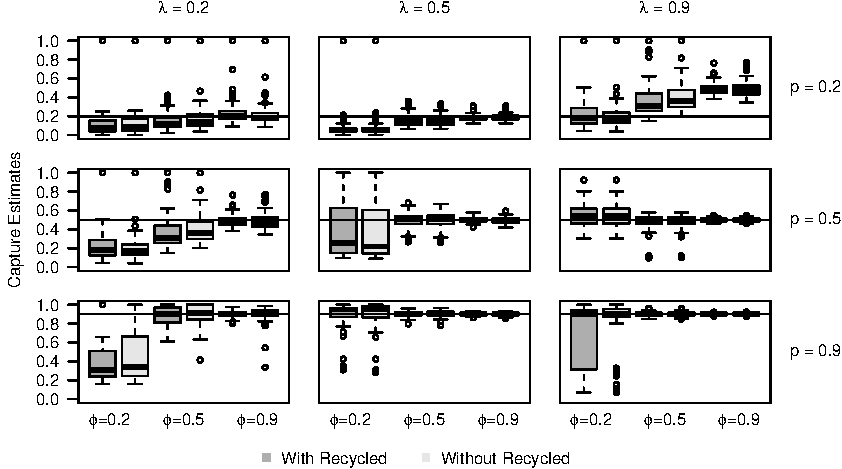
\includegraphics{Appendix_BW_files/figure-latex/figure11_capture_GJSTL5-1.pdf}

\textsc{Web Figure 11:} Boxplots of capture estimates (\(\hat{p}\)) of
100 simulated datasets analyzed with and without the effect of recycled
individuals for population size \(1000\) with \(T_2=1\) for 5 sample times for varying survival (\(\phi=0.2,0.5,0.9\)), capture
(\(p=0.2,0.5,0.9\)), and tag retention (\(\lambda=0.2,0.5,0.9\))
probabilities. The black line indicates the true value of \(p\) used to
simulate the data for each model.

\paragraph{N=1000, T=1, t=7}\label{n1000-t1-t7-1}

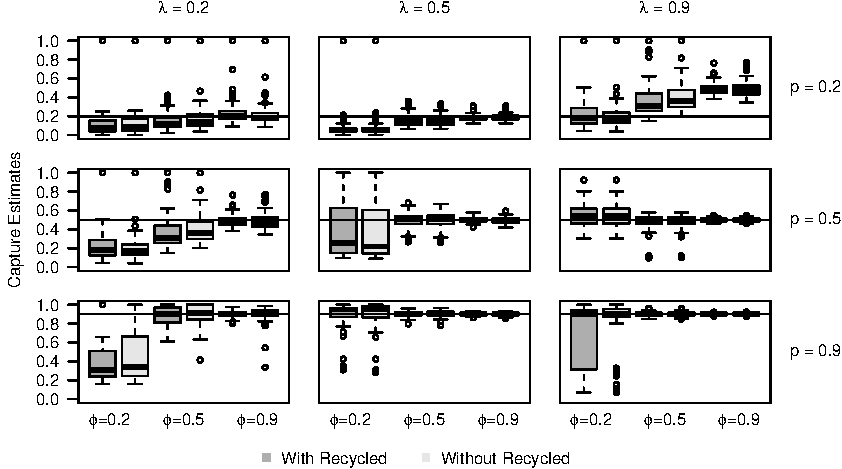
\includegraphics{Appendix_BW_files/figure-latex/figure12_capture_GJSTL6-1.pdf}

\textsc{Web Figure 12:} Boxplots of capture estimates (\(\hat{p}\)) of
100 simulated datasets analyzed with and without the effect of recycled
individuals for population size \(1000\) with \(T_2=1\) for 7 sample times for varying survival (\(\phi=0.2,0.5,0.9\)), capture
(\(p=0.2,0.5,0.9\)), and tag retention (\(\lambda=0.2,0.5,0.9\))
probabilities. The black line indicates the true value of \(p\) used to
simulate the data for each model.

\newpage

\subsection{Tag Retention Estimates}\label{tag-retention-estimates}

\paragraph{N=1000, T=1}\label{n1000-t1-2}

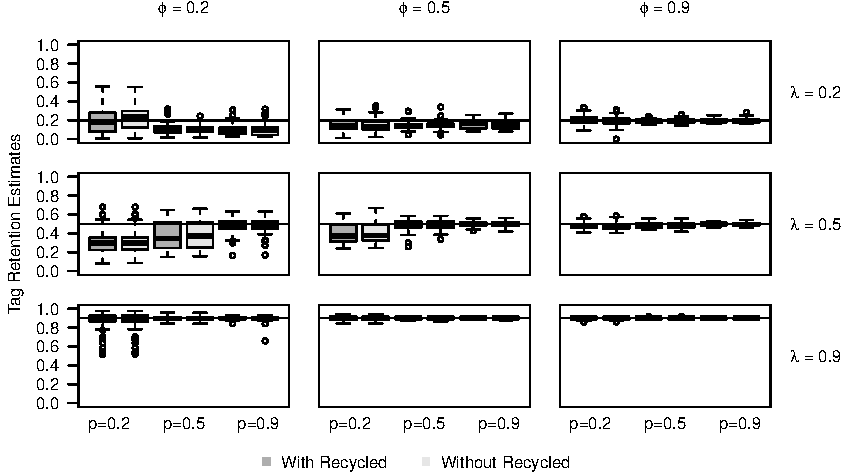
\includegraphics{Appendix_BW_files/figure-latex/figure13_tagretention_GJSTL1-1.pdf}

\textsc{Web Figure 13:} Boxplots of tag retention estimates
(\(\hat{\lambda}\)) of 100 simulated datasets analyzed with and without
the effect of recycled individuals for population size \(1000\) with
\(T_2=1\) with 10 sample times for varying survival
(\(\phi=0.2,0.5,0.9\)), capture (\(p=0.2,0.5,0.9\)), and tag retention
(\(\lambda=0.2,0.5,0.9\)) probabilities. The black line indicates the
true value of \(\lambda\) used to simulate the data for each model.

\textsc{Web Table 9:} Standard Error (SE), Standard Deviation (SD), and
Root Mean Squared Error (RMSE) of tag retention estimates
(\(\hat{\lambda}\)) of 100 simulated datasets analyzed without (R') and
with (R) the effect of recycled individuals with population size
\(N=1000\) with \(T_2=1\) with 10 sample times for varying tag retention
(\(\lambda=0.2,0.5,0.9\)), varying survival probabilities
(\(\phi=0.2,0.5,0.9\)) and varying capture probabilities
(\(p=0.2,0.5,0.9\)).

\begin{table}[ht]
\centering
\begingroup\setlength{\tabcolsep}{12pt}
\scalebox{0.7}{
\begin{tabular}{rrrrrrrrr}
  \hline
$\phi$ & p & $\lambda$ & SE (R') & SE (R) & SD (R') & SD (R) & RMSE (R') & RMSE (R) \\ 
  \hline
0.9 & 0.9 & 0.9 & 0.0051 & 0.0049 & 0.0054 & 0.0054 & 0.0054 & 0.0054 \\ 
  0.9 & 0.9 & 0.5 & 0.0197 & 0.0143 & 0.0188 & 0.0142 & 0.0191 & 0.0144 \\ 
  0.9 & 0.9 & 0.2 & 0.0234 & 0.0152 & 0.0239 & 0.0184 & 0.0242 & 0.0184 \\ 
  0.9 & 0.5 & 0.9 & 0.0065 & 0.0063 & 0.0065 & 0.0061 & 0.0064 & 0.0061 \\ 
  0.9 & 0.5 & 0.5 & 0.0207 & 0.0184 & 0.0324 & 0.0291 & 0.0367 & 0.0314 \\ 
  0.9 & 0.5 & 0.2 & 0.0203 & 0.0178 & 0.0226 & 0.0187 & 0.0243 & 0.0210 \\ 
  0.9 & 0.2 & 0.9 & 0.0114 & 0.0113 & 0.0127 & 0.0129 & 0.0127 & 0.0130 \\ 
  0.9 & 0.2 & 0.5 & 0.0326 & 0.0297 & 0.0408 & 0.0349 & 0.0469 & 0.0417 \\ 
  0.9 & 0.2 & 0.2 & 0.0431 & 0.0386 & 0.0463 & 0.0439 & 0.0462 & 0.0437 \\ 
  0.5 & 0.9 & 0.9 & 0.0093 & 0.0092 & 0.0091 & 0.0091 & 0.0091 & 0.0091 \\ 
  0.5 & 0.9 & 0.5 & 0.0283 & 0.0256 & 0.0294 & 0.0273 & 0.0294 & 0.0272 \\ 
  0.5 & 0.9 & 0.2 & 0.0254 & 0.0260 & 0.0495 & 0.0478 & 0.0655 & 0.0597 \\ 
  0.5 & 0.5 & 0.9 & 0.0123 & 0.0122 & 0.0116 & 0.0115 & 0.0115 & 0.0115 \\ 
  0.5 & 0.5 & 0.5 & 0.0389 & 0.0363 & 0.0489 & 0.0511 & 0.0497 & 0.0517 \\ 
  0.5 & 0.5 & 0.2 & 0.0267 & 0.0250 & 0.0370 & 0.0371 & 0.0652 & 0.0680 \\ 
  0.5 & 0.2 & 0.9 & 0.0224 & 0.0223 & 0.0229 & 0.0224 & 0.0228 & 0.0223 \\ 
  0.5 & 0.2 & 0.5 & 0.0566 & 0.0551 & 0.1072 & 0.1040 & 0.1410 & 0.1421 \\ 
  0.5 & 0.2 & 0.2 & 0.0514 & 0.0480 & 0.0653 & 0.0597 & 0.0838 & 0.0784 \\ 
  0.2 & 0.9 & 0.9 & 0.0171 & 0.0170 & 0.0292 & 0.0165 & 0.0294 & 0.0165 \\ 
  0.2 & 0.9 & 0.5 & 0.0468 & 0.0457 & 0.0692 & 0.0673 & 0.0711 & 0.0686 \\ 
  0.2 & 0.9 & 0.2 & 0.0219 & 0.0234 & 0.0539 & 0.0521 & 0.1168 & 0.1139 \\ 
  0.2 & 0.5 & 0.9 & 0.0240 & 0.0240 & 0.0222 & 0.0220 & 0.0224 & 0.0222 \\ 
  0.2 & 0.5 & 0.5 & 0.0541 & 0.0526 & 0.1386 & 0.1432 & 0.1791 & 0.1866 \\ 
  0.2 & 0.5 & 0.2 & 0.0325 & 0.0323 & 0.0405 & 0.0639 & 0.1047 & 0.1109 \\ 
  0.2 & 0.2 & 0.9 & 0.0513 & 0.0517 & 0.0858 & 0.0857 & 0.0884 & 0.0885 \\ 
  0.2 & 0.2 & 0.5 & 0.0898 & 0.0899 & 0.1087 & 0.1069 & 0.2187 & 0.2229 \\ 
  0.2 & 0.2 & 0.2 & 0.0889 & 0.0824 & 0.1151 & 0.1192 & 0.1159 & 0.1194 \\ 
   \hline
\end{tabular}
}
\endgroup
\end{table}

\newpage

\paragraph{N=100000, T=1}\label{n100000-t1-2}

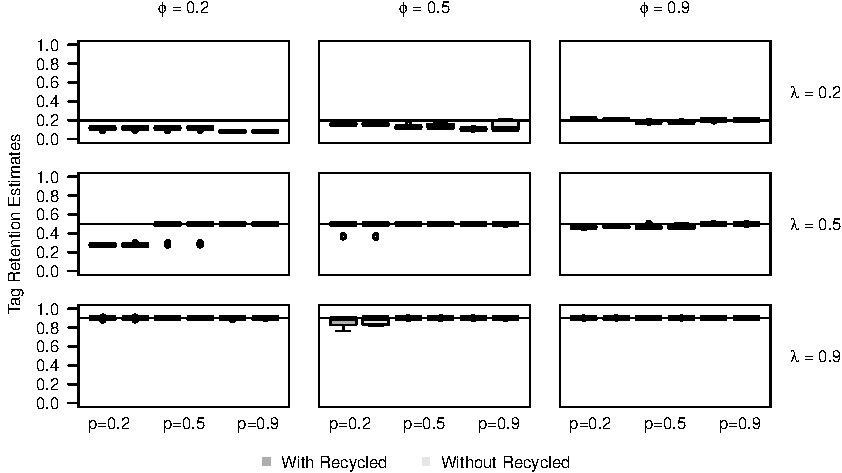
\includegraphics{Appendix_BW_files/figure-latex/figure14_tagretention_GJSTL2-1.pdf}

\textsc{Web Figure 14:} Boxplots of tag retention estimates
(\(\hat{\lambda}\)) of 100 simulated datasets analyzed with and without
the effect of recycled individuals for population size \(100000\) with
\(T_2=1\) with 10 sample times for varying survival
(\(\phi=0.2,0.5,0.9\)), capture (\(p=0.2,0.5,0.9\)), and tag retention
(\(\lambda=0.2,0.5,0.9\)) probabilities. The black line indicates the
true value of \(\lambda\) used to simulate the data for each model.

\textsc{Web Table 10:} Standard Error (SE), Standard Deviation (SD), and
Root Mean Squared Error (RMSE) of tag retention estimates
(\(\hat{\lambda}\)) of 100 simulated datasets analyzed without (R') and
with (R) the effect of recycled individuals with population size
\(N=1000\) with \(T_2=1\) with 10 sample times for varying tag retention
(\(\lambda=0.2,0.5,0.9\)), varying survival probabilities
(\(\phi=0.2,0.5,0.9\)) and varying capture probabilities
(\(p=0.2,0.5,0.9\)).

\begin{table}[ht]
\centering
\begingroup\setlength{\tabcolsep}{12pt}
\scalebox{0.7}{
\begin{tabular}{rrrrrrrrr}
  \hline
$\phi$ & p & $\lambda$ & SE (R') & SE (R) & SD (R') & SD (R) & RMSE (R') & RMSE (R) \\ 
  \hline
0.9 & 0.9 & 0.9 & 0.0051 & 0.0049 & 0.0054 & 0.0054 & 0.0054 & 0.0054 \\ 
  0.9 & 0.9 & 0.5 & 0.0197 & 0.0143 & 0.0188 & 0.0142 & 0.0191 & 0.0144 \\ 
  0.9 & 0.9 & 0.2 & 0.0234 & 0.0152 & 0.0239 & 0.0184 & 0.0242 & 0.0184 \\ 
  0.9 & 0.5 & 0.9 & 0.0065 & 0.0063 & 0.0065 & 0.0061 & 0.0064 & 0.0061 \\ 
  0.9 & 0.5 & 0.5 & 0.0207 & 0.0184 & 0.0324 & 0.0291 & 0.0367 & 0.0314 \\ 
  0.9 & 0.5 & 0.2 & 0.0203 & 0.0178 & 0.0226 & 0.0187 & 0.0243 & 0.0210 \\ 
  0.9 & 0.2 & 0.9 & 0.0114 & 0.0113 & 0.0127 & 0.0129 & 0.0127 & 0.0130 \\ 
  0.9 & 0.2 & 0.5 & 0.0326 & 0.0297 & 0.0408 & 0.0349 & 0.0469 & 0.0417 \\ 
  0.9 & 0.2 & 0.2 & 0.0431 & 0.0386 & 0.0463 & 0.0439 & 0.0462 & 0.0437 \\ 
  0.5 & 0.9 & 0.9 & 0.0093 & 0.0092 & 0.0091 & 0.0091 & 0.0091 & 0.0091 \\ 
  0.5 & 0.9 & 0.5 & 0.0283 & 0.0256 & 0.0294 & 0.0273 & 0.0294 & 0.0272 \\ 
  0.5 & 0.9 & 0.2 & 0.0254 & 0.0260 & 0.0495 & 0.0478 & 0.0655 & 0.0597 \\ 
  0.5 & 0.5 & 0.9 & 0.0123 & 0.0122 & 0.0116 & 0.0115 & 0.0115 & 0.0115 \\ 
  0.5 & 0.5 & 0.5 & 0.0389 & 0.0363 & 0.0489 & 0.0511 & 0.0497 & 0.0517 \\ 
  0.5 & 0.5 & 0.2 & 0.0267 & 0.0250 & 0.0370 & 0.0371 & 0.0652 & 0.0680 \\ 
  0.5 & 0.2 & 0.9 & 0.0224 & 0.0223 & 0.0229 & 0.0224 & 0.0228 & 0.0223 \\ 
  0.5 & 0.2 & 0.5 & 0.0566 & 0.0551 & 0.1072 & 0.1040 & 0.1410 & 0.1421 \\ 
  0.5 & 0.2 & 0.2 & 0.0514 & 0.0480 & 0.0653 & 0.0597 & 0.0838 & 0.0784 \\ 
  0.2 & 0.9 & 0.9 & 0.0171 & 0.0170 & 0.0292 & 0.0165 & 0.0294 & 0.0165 \\ 
  0.2 & 0.9 & 0.5 & 0.0468 & 0.0457 & 0.0692 & 0.0673 & 0.0711 & 0.0686 \\ 
  0.2 & 0.9 & 0.2 & 0.0219 & 0.0234 & 0.0539 & 0.0521 & 0.1168 & 0.1139 \\ 
  0.2 & 0.5 & 0.9 & 0.0240 & 0.0240 & 0.0222 & 0.0220 & 0.0224 & 0.0222 \\ 
  0.2 & 0.5 & 0.5 & 0.0541 & 0.0526 & 0.1386 & 0.1432 & 0.1791 & 0.1866 \\ 
  0.2 & 0.5 & 0.2 & 0.0325 & 0.0323 & 0.0405 & 0.0639 & 0.1047 & 0.1109 \\ 
  0.2 & 0.2 & 0.9 & 0.0513 & 0.0517 & 0.0858 & 0.0857 & 0.0884 & 0.0885 \\ 
  0.2 & 0.2 & 0.5 & 0.0898 & 0.0899 & 0.1087 & 0.1069 & 0.2187 & 0.2229 \\ 
  0.2 & 0.2 & 0.2 & 0.0889 & 0.0824 & 0.1151 & 0.1192 & 0.1159 & 0.1194 \\ 
   \hline
\end{tabular}
}
\endgroup
\end{table}

\newpage

\paragraph{N=1000, T=0.5}\label{n1000-t0.5-2}

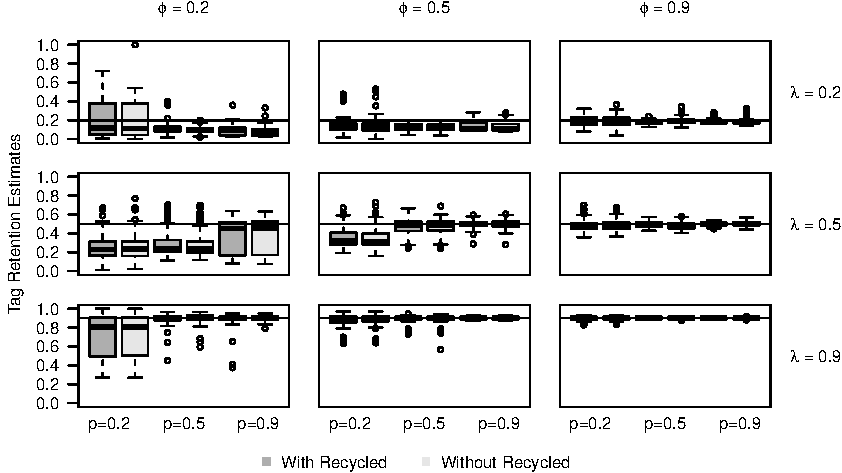
\includegraphics{Appendix_BW_files/figure-latex/figure15_tagretention_GJSTL4-1.pdf}

\textsc{Web Figure 15:} Boxplots of tag retention estimates
(\(\hat{\lambda}\)) of 100 simulated datasets analyzed with and without
the effect of recycled individuals for population size \(1000\) with
\(T_2=0.5\) with 10 sample times for varying survival
(\(\phi=0.2,0.5,0.9\)), capture (\(p=0.2,0.5,0.9\)), and tag retention
(\(\lambda=0.2,0.5,0.9\)) probabilities. The black line indicates the
true value of \(\lambda\) used to simulate the data for each model.

\textsc{Web Table 11:} Standard Error (SE), Standard Deviation (SD), and
Root Mean Squared Error (RMSE) of tag retention estimates
(\(\hat{\lambda}\)) of 100 simulated datasets analyzed without (R') and
with (R) the effect of recycled individuals with population size
\(N=1000\) with \(T_2=0.5\) with 10 sample times for varying tag
retention (\(\lambda=0.2,0.5,0.9\)), varying survival probabilities
(\(\phi=0.2,0.5,0.9\)) and varying capture probabilities
(\(p=0.2,0.5,0.9\)).

\begin{table}[ht]
\centering
\begingroup\setlength{\tabcolsep}{12pt}
\scalebox{0.7}{
\begin{tabular}{rrrrrrrrr}
  \hline
$\phi$ & p & $\lambda$ & SE (R') & SE (R) & SD (R') & SD (R) & RMSE (R') & RMSE (R) \\ 
  \hline
0.9 & 0.9 & 0.9 & 0.0069 & 0.0064 & 0.0067 & 0.0062 & 0.0067 & 0.0063 \\ 
  0.9 & 0.9 & 0.5 & 0.0268 & 0.0185 & 0.0262 & 0.0178 & 0.0262 & 0.0179 \\ 
  0.9 & 0.9 & 0.2 & 0.0186 & 0.0118 & 0.0346 & 0.0229 & 0.0352 & 0.0247 \\ 
  0.9 & 0.5 & 0.9 & 0.0087 & 0.0083 & 0.0081 & 0.0084 & 0.0080 & 0.0084 \\ 
  0.9 & 0.5 & 0.5 & 0.0242 & 0.0256 & 0.0392 & 0.0282 & 0.0429 & 0.0288 \\ 
  0.9 & 0.5 & 0.2 & 0.0253 & 0.0177 & 0.0345 & 0.0192 & 0.0350 & 0.0270 \\ 
  0.9 & 0.2 & 0.9 & 0.0157 & 0.0156 & 0.0168 & 0.0172 & 0.0169 & 0.0174 \\ 
  0.9 & 0.2 & 0.5 & 0.0421 & 0.0370 & 0.0602 & 0.0584 & 0.0617 & 0.0604 \\ 
  0.9 & 0.2 & 0.2 & 0.0498 & 0.0452 & 0.0538 & 0.0492 & 0.0547 & 0.0499 \\ 
  0.5 & 0.9 & 0.9 & 0.0129 & 0.0126 & 0.0130 & 0.0128 & 0.0130 & 0.0128 \\ 
  0.5 & 0.9 & 0.5 & 0.0387 & 0.0342 & 0.0446 & 0.0420 & 0.0445 & 0.0418 \\ 
  0.5 & 0.9 & 0.2 & 0.0170 & 0.0172 & 0.0432 & 0.0508 & 0.0867 & 0.0835 \\ 
  0.5 & 0.5 & 0.9 & 0.0172 & 0.0170 & 0.0519 & 0.0379 & 0.0532 & 0.0387 \\ 
  0.5 & 0.5 & 0.5 & 0.0510 & 0.0435 & 0.0865 & 0.0964 & 0.0922 & 0.1040 \\ 
  0.5 & 0.5 & 0.2 & 0.0277 & 0.0253 & 0.0372 & 0.0385 & 0.0839 & 0.0812 \\ 
  0.5 & 0.2 & 0.9 & 0.0340 & 0.0340 & 0.0696 & 0.0659 & 0.0731 & 0.0699 \\ 
  0.5 & 0.2 & 0.5 & 0.0627 & 0.0623 & 0.1117 & 0.1002 & 0.1838 & 0.1766 \\ 
  0.5 & 0.2 & 0.2 & 0.0563 & 0.0597 & 0.0879 & 0.0909 & 0.1079 & 0.1024 \\ 
  0.2 & 0.9 & 0.9 & 0.0240 & 0.0241 & 0.0269 & 0.0792 & 0.0268 & 0.0801 \\ 
  0.2 & 0.9 & 0.5 & 0.0510 & 0.0477 & 0.1798 & 0.1830 & 0.2166 & 0.2237 \\ 
  0.2 & 0.9 & 0.2 & 0.0252 & 0.0219 & 0.0497 & 0.0564 & 0.1273 & 0.1229 \\ 
  0.2 & 0.5 & 0.9 & 0.0340 & 0.0341 & 0.0554 & 0.0625 & 0.0555 & 0.0629 \\ 
  0.2 & 0.5 & 0.5 & 0.0545 & 0.0537 & 0.1572 & 0.1479 & 0.2558 & 0.2533 \\ 
  0.2 & 0.5 & 0.2 & 0.0346 & 0.0360 & 0.0376 & 0.0723 & 0.1056 & 0.1104 \\ 
  0.2 & 0.2 & 0.9 & 0.0897 & 0.0907 & 0.2184 & 0.2189 & 0.2911 & 0.2890 \\ 
  0.2 & 0.2 & 0.5 & 0.0930 & 0.0911 & 0.1403 & 0.1252 & 0.2771 & 0.2813 \\ 
  0.2 & 0.2 & 0.2 & 0.0855 & 0.0907 & 0.1852 & 0.1774 & 0.1843 & 0.1766 \\ 
   \hline
\end{tabular}
}
\endgroup
\end{table}

\newpage

\paragraph{N=100000, T=0.5}\label{n100000-t0.5-2}

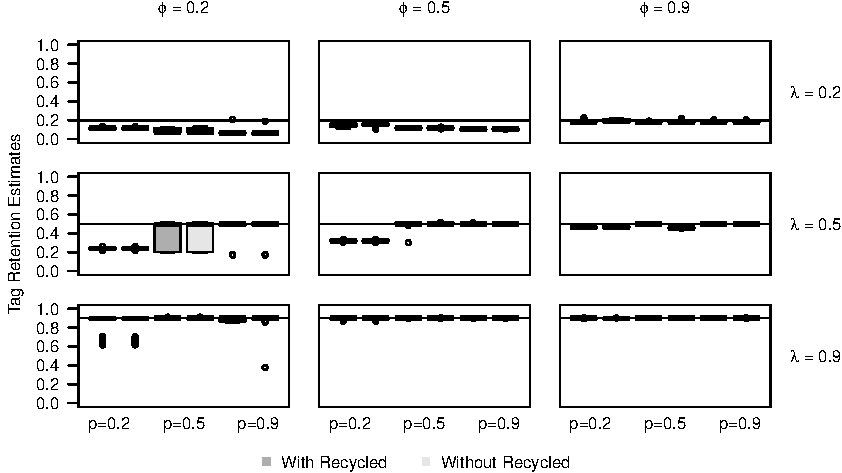
\includegraphics{Appendix_BW_files/figure-latex/figure16_tagretention_GJSTL3-1.pdf}

\textsc{Web Figure 16:} Boxplots of tag retention estimates
(\(\hat{\lambda}\)) of 100 simulated datasets analyzed with and without
the effect of recycled individuals for population size \(100000\) with
\(T_2=0.5\) with 10 sample times for varying survival
(\(\phi=0.2,0.5,0.9\)), capture (\(p=0.2,0.5,0.9\)), and tag retention
(\(\lambda=0.2,0.5,0.9\)) probabilities. The black line indicates the
true value of \(\lambda\) used to simulate the data for each model.

\textsc{Web Table 12:} Standard Error (SE), Standard Deviation (SD), and
Root Mean Squared Error (RMSE) of tag retention estimates
(\(\hat{\lambda}\)) of 100 simulated datasets analyzed without (R') and
with (R) the effect of recycled individuals with population size
\(N=100000\) with \(T_2=0.5\) with 10 sample times for varying tag
retention (\(\lambda=0.2,0.5,0.9\)), varying survival probabilities
(\(\phi=0.2,0.5,0.9\)) and varying capture probabilities
(\(p=0.2,0.5,0.9\)).

\begin{table}[ht]
\centering
\begingroup\setlength{\tabcolsep}{12pt}
\scalebox{0.7}{
\begin{tabular}{rrrrrrrrr}
  \hline
$\phi$ & p & $\lambda$ & SE (R') & SE (R) & SD (R') & SD (R) & RMSE (R') & RMSE (R) \\ 
  \hline
0.9 & 0.9 & 0.9 & 0.0007 & 0.0006 & 0.0007 & 0.0006 & 0.0007 & 0.0006 \\ 
  0.9 & 0.9 & 0.5 & 0.0027 & 0.0019 & 0.0028 & 0.0019 & 0.0028 & 0.0020 \\ 
  0.9 & 0.9 & 0.2 & 0.0016 & 0.0008 & 0.0064 & 0.0033 & 0.0177 & 0.0190 \\ 
  0.9 & 0.5 & 0.9 & 0.0009 & 0.0008 & 0.0008 & 0.0008 & 0.0008 & 0.0008 \\ 
  0.9 & 0.5 & 0.5 & 0.0017 & 0.0029 & 0.0018 & 0.0026 & 0.0431 & 0.0026 \\ 
  0.9 & 0.5 & 0.2 & 0.0024 & 0.0017 & 0.0045 & 0.0017 & 0.0171 & 0.0169 \\ 
  0.9 & 0.2 & 0.9 & 0.0016 & 0.0015 & 0.0019 & 0.0018 & 0.0035 & 0.0019 \\ 
  0.9 & 0.2 & 0.5 & 0.0036 & 0.0033 & 0.0054 & 0.0036 & 0.0330 & 0.0370 \\ 
  0.9 & 0.2 & 0.2 & 0.0052 & 0.0046 & 0.0148 & 0.0061 & 0.0155 & 0.0166 \\ 
  0.5 & 0.9 & 0.9 & 0.0013 & 0.0013 & 0.0013 & 0.0013 & 0.0013 & 0.0013 \\ 
  0.5 & 0.9 & 0.5 & 0.0039 & 0.0034 & 0.0038 & 0.0033 & 0.0038 & 0.0033 \\ 
  0.5 & 0.9 & 0.2 & 0.0014 & 0.0012 & 0.0014 & 0.0011 & 0.0951 & 0.0950 \\ 
  0.5 & 0.5 & 0.9 & 0.0017 & 0.0017 & 0.0016 & 0.0015 & 0.0016 & 0.0015 \\ 
  0.5 & 0.5 & 0.5 & 0.0054 & 0.0050 & 0.0053 & 0.0207 & 0.0053 & 0.0207 \\ 
  0.5 & 0.5 & 0.2 & 0.0031 & 0.0027 & 0.0029 & 0.0027 & 0.0819 & 0.0816 \\ 
  0.5 & 0.2 & 0.9 & 0.0032 & 0.0031 & 0.0093 & 0.0079 & 0.0101 & 0.0082 \\ 
  0.5 & 0.2 & 0.5 & 0.0056 & 0.0055 & 0.0053 & 0.0051 & 0.1794 & 0.1790 \\ 
  0.5 & 0.2 & 0.2 & 0.0064 & 0.0061 & 0.0151 & 0.0175 & 0.0504 & 0.0536 \\ 
  0.2 & 0.9 & 0.9 & 0.0026 & 0.0027 & 0.0537 & 0.0174 & 0.0550 & 0.0212 \\ 
  0.2 & 0.9 & 0.5 & 0.0060 & 0.0058 & 0.1104 & 0.1171 & 0.1182 & 0.1269 \\ 
  0.2 & 0.9 & 0.2 & 0.0031 & 0.0028 & 0.0129 & 0.0147 & 0.1360 & 0.1359 \\ 
  0.2 & 0.5 & 0.9 & 0.0033 & 0.0033 & 0.0032 & 0.0032 & 0.0032 & 0.0032 \\ 
  0.2 & 0.5 & 0.5 & 0.0072 & 0.0068 & 0.1502 & 0.1518 & 0.1932 & 0.2040 \\ 
  0.2 & 0.5 & 0.2 & 0.0046 & 0.0044 & 0.0200 & 0.0192 & 0.1130 & 0.1120 \\ 
  0.2 & 0.2 & 0.9 & 0.0080 & 0.0082 & 0.0922 & 0.0985 & 0.1018 & 0.1107 \\ 
  0.2 & 0.2 & 0.5 & 0.0090 & 0.0089 & 0.0075 & 0.0075 & 0.2603 & 0.2601 \\ 
  0.2 & 0.2 & 0.2 & 0.0092 & 0.0091 & 0.0070 & 0.0070 & 0.0854 & 0.0850 \\ 
   \hline
\end{tabular}
}
\endgroup
\end{table}

\newpage

\paragraph{N=1000, T=1, t=5}\label{n1000-t1-t5-2}

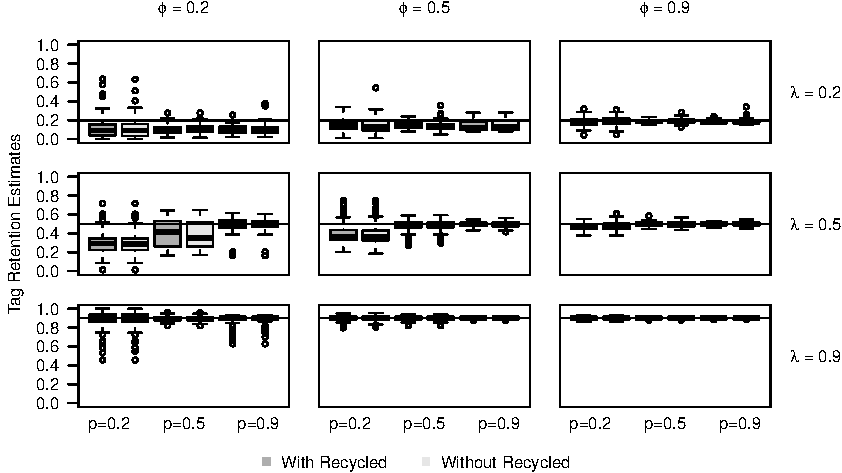
\includegraphics{Appendix_BW_files/figure-latex/figure17_tagretention_GJSTL5-1.pdf}

\textsc{Web Figure 17:} Boxplots of tag retention estimates
(\(\hat{\lambda}\)) of 100 simulated datasets analyzed with and without
the effect of recycled individuals for population size \(1000\) with
\(T_2=1\) for 5 sample times for varying survival
(\(\phi=0.2,0.5,0.9\)), capture (\(p=0.2,0.5,0.9\)), and tag retention
(\(\lambda=0.2,0.5,0.9\)) probabilities. The black line indicates the
true value of \(\lambda\) used to simulate the data for each model.

\paragraph{N=1000, T=1, t=7}\label{n1000-t1-t7-2}

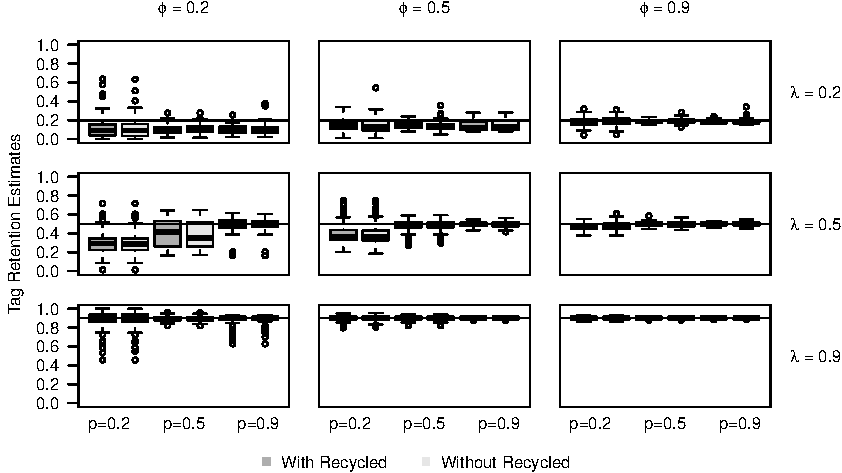
\includegraphics{Appendix_BW_files/figure-latex/figure18_tagretention_GJSTL6-1.pdf}

\textsc{Web Figure 18:} Boxplots of tag retention estimates
(\(\hat{\lambda}\)) of 100 simulated datasets analyzed with and without
the effect of recycled individuals for population size \(1000\) with
\(T_2=1\) for 7 sample times for varying survival
(\(\phi=0.2,0.5,0.9\)), capture (\(p=0.2,0.5,0.9\)), and tag retention
(\(\lambda=0.2,0.5,0.9\)) probabilities. The black line indicates the
true value of \(\lambda\) used to simulate the data for each model.

\newpage

\subsection{Super-Population Size
Estimates}\label{super-population-size-estimates}

\paragraph{N=1000, T=1}\label{n1000-t1-3}

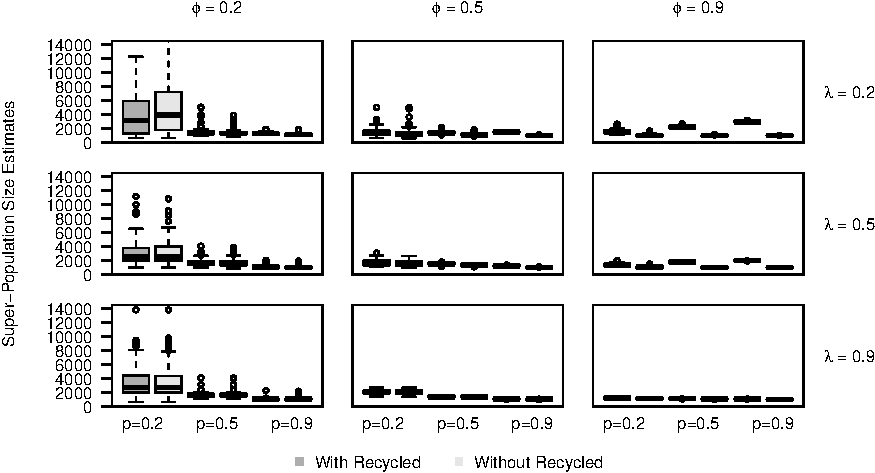
\includegraphics{Appendix_BW_files/figure-latex/figure19_superN_GJSTL1-1.pdf}

\textsc{Web Figure 19:} Boxplots of super-population size estimates
(\(N\)) of 100 simulated datasets analyzed with and without the effect
of recycled individuals for population size \(1000\) with \(T_2=1\) with
10 sample times for varying survival (\(\phi=0.2,0.5,0.9\)), capture
(\(p=0.2,0.5,0.9\)), and tag retention (\(\lambda=0.2,0.5,0.9\))
probabilities. The black line indicates the true value of \(N\) used to
simulate the data for each model.

\textsc{Web Table 13:} Standard Error (SE), Standard Deviation (SD), and
Root Mean Squared Error (RMSE) of super-population size estimates
(\(N\)) of 100 simulated datasets analyzed without (R') and with (R) the
effect of recycled individuals with population size \(N=1000\) with
\(T_2=1\) with 10 sample times for varying tag retention
(\(\lambda=0.2,0.5,0.9\)), varying survival probabilities
(\(\phi=0.2,0.5,0.9\)) and varying capture probabilities
(\(p=0.2,0.5,0.9\)).

\begin{table}[ht]
\centering
\begingroup\setlength{\tabcolsep}{12pt}
\scalebox{0.7}{
\begin{tabular}{rrrrrrrrr}
  \hline
$\phi$ & p & $\lambda$ & SE (R') & SE (R) & SD (R') & SD (R) & RMSE (R') & RMSE (R) \\ 
  \hline
0.9 & 0.9 & 0.9 & 50.5 & 50.5 & 4.0 & 11.1 & 10.8 & 114.5 \\ 
  0.9 & 0.9 & 0.5 & 50.5 & 50.5 & 5.8 & 33.0 & 11.0 & 1037.9 \\ 
  0.9 & 0.9 & 0.2 & 49.6 & 49.6 & 10.5 & 75.8 & 12.0 & 1980.5 \\ 
  0.9 & 0.5 & 0.9 & 50.5 & 50.5 & 19.0 & 21.9 & 80.8 & 164.5 \\ 
  0.9 & 0.5 & 0.5 & 50.5 & 50.5 & 54.5 & 82.5 & 68.2 & 801.9 \\ 
  0.9 & 0.5 & 0.2 & 50.5 & 50.5 & 34.9 & 112.9 & 37.0 & 1266.4 \\ 
  0.9 & 0.2 & 0.9 & 49.8 & 49.8 & 74.2 & 80.3 & 192.9 & 245.4 \\ 
  0.9 & 0.2 & 0.5 & 50.5 & 50.5 & 130.0 & 160.7 & 156.0 & 477.6 \\ 
  0.9 & 0.2 & 0.2 & 49.6 & 50.5 & 173.7 & 290.1 & 179.3 & 687.8 \\ 
  0.5 & 0.9 & 0.9 & 50.5 & 50.5 & 12.0 & 12.7 & 49.1 & 64.7 \\ 
  0.5 & 0.9 & 0.5 & 50.5 & 50.5 & 16.9 & 28.4 & 48.0 & 284.1 \\ 
  0.5 & 0.9 & 0.2 & 49.6 & 49.6 & 34.7 & 57.0 & 44.2 & 527.3 \\ 
  0.5 & 0.5 & 0.9 & 50.5 & 50.5 & 61.6 & 61.6 & 411.9 & 424.5 \\ 
  0.5 & 0.5 & 0.5 & 50.4 & 50.4 & 85.0 & 95.9 & 388.2 & 576.5 \\ 
  0.5 & 0.5 & 0.2 & 50.5 & 50.5 & 108.7 & 132.5 & 157.8 & 443.4 \\ 
  0.5 & 0.2 & 0.9 & 49.4 & 49.4 & 276.4 & 273.7 & 1152.3 & 1149.4 \\ 
  0.5 & 0.2 & 0.5 & 50.5 & 50.5 & 417.9 & 445.8 & 723.5 & 816.6 \\ 
  0.5 & 0.2 & 0.2 & 49.4 & 49.4 & 710.4 & 587.7 & 801.9 & 760.4 \\ 
  0.2 & 0.9 & 0.9 & 50.5 & 50.5 & 158.2 & 132.9 & 184.1 & 156.7 \\ 
  0.2 & 0.9 & 0.5 & 50.8 & 50.5 & 176.7 & 165.7 & 194.4 & 214.2 \\ 
  0.2 & 0.9 & 0.2 & 50.3 & 50.3 & 161.5 & 164.5 & 226.2 & 346.0 \\ 
  0.2 & 0.5 & 0.9 & 50.5 & 50.5 & 426.7 & 362.3 & 815.9 & 763.0 \\ 
  0.2 & 0.5 & 0.5 & 50.5 & 50.5 & 624.0 & 582.9 & 973.6 & 954.5 \\ 
  0.2 & 0.5 & 0.2 & 50.5 & 50.5 & 423.4 & 784.3 & 583.8 & 993.3 \\ 
  0.2 & 0.2 & 0.9 & 50.5 & 50.5 & 2517.1 & 2485.1 & 3651.5 & 3662.1 \\ 
  0.2 & 0.2 & 0.5 & 50.1 & 50.1 & 1852.7 & 1877.8 & 2882.2 & 2866.4 \\ 
  0.2 & 0.2 & 0.2 & 49.1 & 49.1 & 8456.1 & 3760.5 & 9651.8 & 5001.5 \\ 
   \hline
\end{tabular}
}
\endgroup
\end{table}

\newpage

\paragraph{N=100000, T=0.5}\label{n100000-t0.5-3}

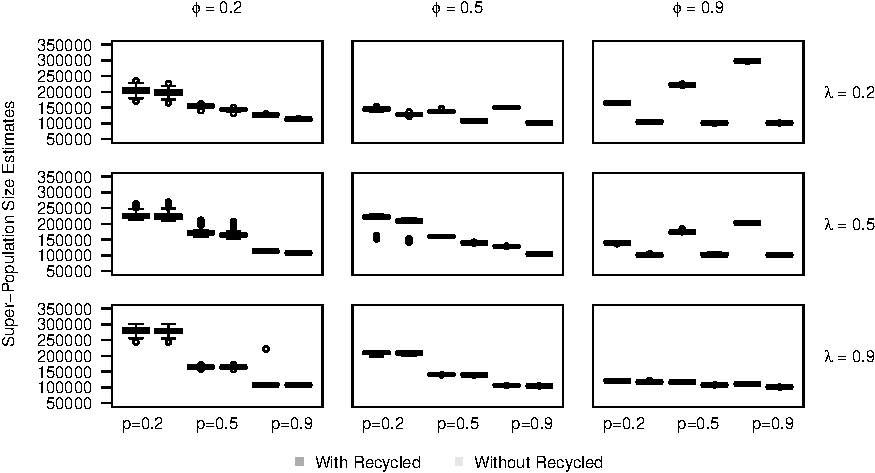
\includegraphics{Appendix_BW_files/figure-latex/figure20_superN_GJSTL2-1.pdf}

\textsc{Web Figure 20:} Boxplots of super-population size estimates
(\(N\)) of 100 simulated datasets analyzed with and without the effect
of recycled individuals for population size \(100000\) with \(T_2=1\)
with 10 sample times for varying survival (\(\phi=0.2,0.5,0.9\)),
capture (\(p=0.2,0.5,0.9\)), and tag retention (\(\lambda=0.2,0.5,0.9\))
probabilities. The black line indicates the true value of \(N\) used to
simulate the data for each model.

\textsc{Web Table 14:} Standard Error (SE), Standard Deviation (SD), and
Root Mean Squared Error (RMSE) of super-population size estimates
(\(N\)) of 100 simulated datasets analyzed without (R') and with (R) the
effect of recycled individuals with population size \(N=100000\) with
\(T_2=1\) with 10 sample times for varying tag retention
(\(\lambda=0.2,0.5,0.9\)), varying survival probabilities
(\(\phi=0.2,0.5,0.9\)) and varying capture probabilities
(\(p=0.2,0.5,0.9\)).

\begin{table}[ht]
\centering
\begingroup\setlength{\tabcolsep}{12pt}
\scalebox{0.7}{
\begin{tabular}{rrrrrrrrr}
  \hline
$\phi$ & p & $\lambda$ & SE (R') & SE (R) & SD (R') & SD (R) & RMSE (R') & RMSE (R) \\ 
  \hline
0.9 & 0.9 & 0.9 & 42.1 & 42.1 & 38.9 & 107.6 & 988.1 & 11361.8 \\ 
  0.9 & 0.9 & 0.5 & 37.8 & 37.8 & 48.3 & 355.4 & 982.7 & 103591.7 \\ 
  0.9 & 0.9 & 0.2 & 38.5 & 38.5 & 135.9 & 662.0 & 982.7 & 198249.4 \\ 
  0.9 & 0.5 & 0.9 & 37.9 & 37.9 & 175.4 & 211.2 & 7994.0 & 16488.3 \\ 
  0.9 & 0.5 & 0.5 & 37.9 & 37.9 & 3572.1 & 3521.2 & 5471.0 & 74619.3 \\ 
  0.9 & 0.5 & 0.2 & 41.4 & 41.4 & 296.0 & 800.3 & 712.4 & 122405.8 \\ 
  0.9 & 0.2 & 0.9 & 49.4 & 49.4 & 775.8 & 564.4 & 16686.3 & 21184.5 \\ 
  0.9 & 0.2 & 0.5 & 50.5 & 50.5 & 1545.3 & 993.9 & 1910.3 & 40081.3 \\ 
  0.9 & 0.2 & 0.2 & 50.5 & 50.5 & 1270.1 & 1737.6 & 5261.2 & 64349.6 \\ 
  0.5 & 0.9 & 0.9 & 50.5 & 50.5 & 109.5 & 117.8 & 4937.2 & 6525.9 \\ 
  0.5 & 0.9 & 0.5 & 50.5 & 50.5 & 173.4 & 267.0 & 4934.9 & 28655.8 \\ 
  0.5 & 0.9 & 0.2 & 37.3 & 37.3 & 1600.4 & 323.9 & 2719.0 & 50378.1 \\ 
  0.5 & 0.5 & 0.9 & 50.5 & 50.5 & 595.7 & 598.0 & 40018.0 & 41403.6 \\ 
  0.5 & 0.5 & 0.5 & 37.9 & 37.9 & 934.1 & 1019.7 & 40127.1 & 59803.7 \\ 
  0.5 & 0.5 & 0.2 & 38.1 & 38.1 & 3118.2 & 3462.6 & 9395.9 & 39297.7 \\ 
  0.5 & 0.2 & 0.9 & 48.9 & 48.9 & 3926.0 & 3936.0 & 109240.3 & 109983.6 \\ 
  0.5 & 0.2 & 0.5 & 42.1 & 42.1 & 18455.0 & 17443.4 & 106660.8 & 120015.2 \\ 
  0.5 & 0.2 & 0.2 & 50.5 & 50.5 & 2571.6 & 2768.5 & 28853.1 & 45396.0 \\ 
  0.2 & 0.9 & 0.9 & 37.9 & 37.9 & 428.2 & 15996.7 & 7973.9 & 19083.5 \\ 
  0.2 & 0.9 & 0.5 & 38.3 & 38.3 & 772.7 & 817.7 & 7954.7 & 13739.3 \\ 
  0.2 & 0.9 & 0.2 & 38.1 & 38.1 & 897.2 & 969.9 & 13086.8 & 27825.1 \\ 
  0.2 & 0.5 & 0.9 & 43.6 & 43.6 & 2729.4 & 2724.0 & 64215.6 & 64466.8 \\ 
  0.2 & 0.5 & 0.5 & 38.1 & 38.1 & 12500.3 & 14199.0 & 70108.9 & 77289.2 \\ 
  0.2 & 0.5 & 0.2 & 42.0 & 42.0 & 2572.1 & 2739.3 & 44049.6 & 55230.3 \\ 
  0.2 & 0.2 & 0.9 & 42.1 & 42.1 & 10707.4 & 10726.6 & 178913.1 & 179098.6 \\ 
  0.2 & 0.2 & 0.5 & 50.5 & 50.5 & 12705.6 & 11900.4 & 125943.1 & 128430.9 \\ 
  0.2 & 0.2 & 0.2 & 50.5 & 50.5 & 9921.4 & 10271.3 & 99244.6 & 105891.3 \\ 
   \hline
\end{tabular}
}
\endgroup
\end{table}

\newpage

\paragraph{N=1000, T=0.5}\label{n1000-t0.5-3}

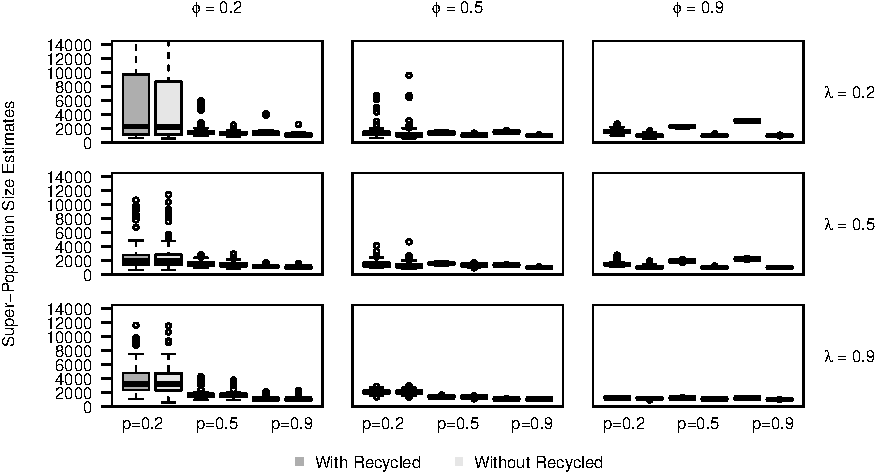
\includegraphics{Appendix_BW_files/figure-latex/figure21_superN_GJSTL4-1.pdf}

\textsc{Web Figure 21:} Boxplots of super-population size estimates
(\(N\)) of 100 simulated datasets analyzed with and without the effect
of recycled individuals for population size \(1000\) with \(T_2=0.5\)
with 10 sample times for varying survival (\(\phi=0.2,0.5,0.9\)),
capture (\(p=0.2,0.5,0.9\)), and tag retention (\(\lambda=0.2,0.5,0.9\))
probabilities. The black line indicates the true value of \(N\) used to
simulate the data for each model.

\textsc{Web Table 15:} Standard Error (SE), Standard Deviation (SD), and
Root Mean Squared Error (RMSE) of super-population size estimates
(\(N\)) of 100 simulated datasets analyzed without (R') and with (R) the
effect of recycled individuals with population size \(N=1000\) with
\(T_2=0.5\) with 10 sample times for varying tag retention
(\(\lambda=0.2,0.5,0.9\)), varying survival probabilities
(\(\phi=0.2,0.5,0.9\)) and varying capture probabilities
(\(p=0.2,0.5,0.9\)).

\begin{table}[ht]
\centering
\begingroup\setlength{\tabcolsep}{12pt}
\scalebox{0.7}{
\begin{tabular}{rrrrrrrrr}
  \hline
$\phi$ & p & $\lambda$ & SE (R') & SE (R) & SD (R') & SD (R) & RMSE (R') & RMSE (R) \\ 
  \hline
0.9 & 0.9 & 0.9 & 50.5 & 50.5 & 4.1 & 13.6 & 98990.4 & 98793.7 \\ 
  0.9 & 0.9 & 0.5 & 50.5 & 50.5 & 7.1 & 39.2 & 98990.7 & 97760.7 \\ 
  0.9 & 0.9 & 0.2 & 50.5 & 50.5 & 13.0 & 66.0 & 98996.6 & 96870.5 \\ 
  0.9 & 0.5 & 0.9 & 50.5 & 50.5 & 19.3 & 28.0 & 98920.9 & 98760.1 \\ 
  0.9 & 0.5 & 0.5 & 50.3 & 50.3 & 62.8 & 89.9 & 98963.0 & 98058.6 \\ 
  0.9 & 0.5 & 0.2 & 50.5 & 50.5 & 54.8 & 91.8 & 98984.5 & 97710.5 \\ 
  0.9 & 0.2 & 0.9 & 50.5 & 50.5 & 68.2 & 75.3 & 98813.8 & 98717.0 \\ 
  0.9 & 0.2 & 0.5 & 50.5 & 50.5 & 211.3 & 275.9 & 98886.7 & 98472.5 \\ 
  0.9 & 0.2 & 0.2 & 50.5 & 50.5 & 197.3 & 294.3 & 98961.1 & 98383.8 \\ 
  0.5 & 0.9 & 0.9 & 50.5 & 50.5 & 12.6 & 13.8 & 98952.5 & 98906.8 \\ 
  0.5 & 0.9 & 0.5 & 50.5 & 50.5 & 20.8 & 29.6 & 98955.0 & 98645.7 \\ 
  0.5 & 0.9 & 0.2 & 50.4 & 50.4 & 35.9 & 62.7 & 98981.0 & 98437.8 \\ 
  0.5 & 0.5 & 0.9 & 50.3 & 50.3 & 73.0 & 70.3 & 98608.8 & 98566.8 \\ 
  0.5 & 0.5 & 0.5 & 49.3 & 49.3 & 135.1 & 179.0 & 98657.1 & 98440.0 \\ 
  0.5 & 0.5 & 0.2 & 50.5 & 50.5 & 89.9 & 118.4 & 98932.9 & 98602.1 \\ 
  0.5 & 0.2 & 0.9 & 50.0 & 50.0 & 293.9 & 276.7 & 97899.1 & 97877.0 \\ 
  0.5 & 0.2 & 0.5 & 49.7 & 49.7 & 526.1 & 532.8 & 98627.1 & 98483.6 \\ 
  0.5 & 0.2 & 0.2 & 49.4 & 49.3 & 1206.1 & 1205.4 & 98637.9 & 98389.6 \\ 
  0.2 & 0.9 & 0.9 & 50.5 & 50.5 & 184.9 & 200.8 & 98901.6 & 98873.5 \\ 
  0.2 & 0.9 & 0.5 & 50.3 & 50.3 & 130.2 & 119.9 & 98908.3 & 98831.8 \\ 
  0.2 & 0.9 & 0.2 & 49.7 & 49.7 & 194.6 & 410.9 & 98872.1 & 98639.7 \\ 
  0.2 & 0.5 & 0.9 & 50.5 & 50.5 & 449.9 & 540.4 & 98331.1 & 98283.4 \\ 
  0.2 & 0.5 & 0.5 & 50.2 & 50.2 & 357.5 & 410.7 & 98531.2 & 98447.0 \\ 
  0.2 & 0.5 & 0.2 & 50.5 & 50.5 & 262.1 & 903.0 & 98660.0 & 98354.8 \\ 
  0.2 & 0.2 & 0.9 & 49.0 & 49.0 & 2151.8 & 2035.6 & 96164.6 & 96153.8 \\ 
  0.2 & 0.2 & 0.5 & 48.9 & 48.9 & 2042.4 & 2077.0 & 97454.8 & 97469.4 \\ 
  0.2 & 0.2 & 0.2 & 49.1 & 46.7 & 11541.5 & 11170.7 & 94078.0 & 93726.1 \\ 
   \hline
\end{tabular}
}
\endgroup
\end{table}

\newpage

\paragraph{N=100000, T=0.5}\label{n100000-t0.5-4}

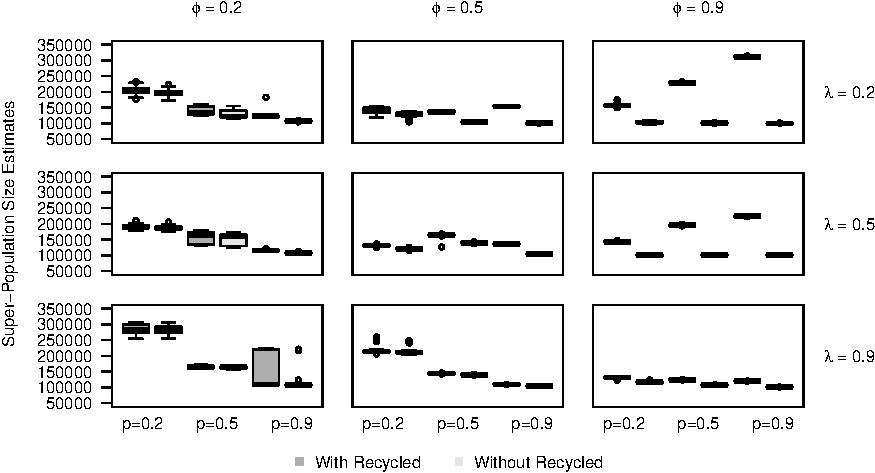
\includegraphics{Appendix_BW_files/figure-latex/figure22_superN_GJSTL3-1.pdf}

\textsc{Web Figure 22:} Boxplots of super-population size estimates
(\(N\)) of 100 simulated datasets analyzed with and without the effect
of recycled individuals for population size \(100000\) with \(T_2=0.5\)
with 10 sample times for varying survival (\(\phi=0.2,0.5,0.9\)),
capture (\(p=0.2,0.5,0.9\)), and tag retention (\(\lambda=0.2,0.5,0.9\))
probabilities. The black line indicates the true value of \(N\) used to
simulate the data for each model.

\textsc{Web Table 16:} Standard Error (SE), Standard Deviation (SD), and
Root Mean Squared Error (RMSE) of super-population size estimates
(\(N\)) of 100 simulated datasets analyzed without (R') and with (R) the
effect of recycled individuals with population size \(N=100000\) with
\(T_2=0.5\) with 10 sample times for varying tag retention
(\(\lambda=0.2,0.5,0.9\)), varying survival probabilities
(\(\phi=0.2,0.5,0.9\)) and varying capture probabilities
(\(p=0.2,0.5,0.9\)).

\begin{table}[ht]
\centering
\begingroup\setlength{\tabcolsep}{12pt}
\scalebox{0.7}{
\begin{tabular}{rrrrrrrrr}
  \hline
$\phi$ & p & $\lambda$ & SE (R') & SE (R) & SD (R') & SD (R) & RMSE (R') & RMSE (R) \\ 
  \hline
0.9 & 0.9 & 0.9 & 50.5 & 50.5 & 38.2 & 154.8 & 996.5 & 20737.8 \\ 
  0.9 & 0.9 & 0.5 & 50.5 & 50.5 & 65.0 & 424.6 & 994.0 & 124165.7 \\ 
  0.9 & 0.9 & 0.2 & 50.5 & 50.5 & 332.4 & 698.0 & 384.3 & 211677.2 \\ 
  0.9 & 0.5 & 0.9 & 50.5 & 50.5 & 150.6 & 230.0 & 8000.3 & 24281.5 \\ 
  0.9 & 0.5 & 0.5 & 50.5 & 50.5 & 188.6 & 778.9 & 716.8 & 96173.9 \\ 
  0.9 & 0.5 & 0.2 & 50.5 & 50.5 & 429.5 & 836.9 & 674.7 & 129334.3 \\ 
  0.9 & 0.2 & 0.9 & 50.5 & 50.5 & 1869.8 & 2206.8 & 16707.2 & 31391.7 \\ 
  0.9 & 0.2 & 0.5 & 50.5 & 50.5 & 1359.9 & 1149.9 & 1675.6 & 43537.0 \\ 
  0.9 & 0.2 & 0.2 & 50.5 & 50.5 & 3394.6 & 3112.9 & 5123.0 & 57428.7 \\ 
  0.5 & 0.9 & 0.9 & 50.5 & 50.5 & 120.8 & 142.7 & 4955.3 & 9575.2 \\ 
  0.5 & 0.9 & 0.5 & 50.5 & 50.5 & 187.0 & 302.3 & 4914.5 & 35599.2 \\ 
  0.5 & 0.9 & 0.2 & 50.5 & 50.5 & 168.8 & 359.0 & 679.4 & 54183.0 \\ 
  0.5 & 0.5 & 0.9 & 50.5 & 50.5 & 542.8 & 560.4 & 40070.0 & 44111.9 \\ 
  0.5 & 0.5 & 0.5 & 50.7 & 50.7 & 1005.8 & 4079.9 & 40103.5 & 64909.0 \\ 
  0.5 & 0.5 & 0.2 & 50.5 & 50.5 & 669.8 & 911.8 & 4448.1 & 37200.1 \\ 
  0.5 & 0.2 & 0.9 & 50.5 & 50.5 & 12143.1 & 10053.7 & 116273.8 & 116900.2 \\ 
  0.5 & 0.2 & 0.5 & 50.5 & 50.5 & 1854.1 & 1903.6 & 21073.9 & 31154.4 \\ 
  0.5 & 0.2 & 0.2 & 50.5 & 50.5 & 7436.9 & 9739.0 & 27781.3 & 43358.6 \\ 
  0.2 & 0.9 & 0.9 & 50.5 & 50.5 & 45500.3 & 53655.2 & 55134.4 & 71471.1 \\ 
  0.2 & 0.9 & 0.5 & 49.5 & 49.5 & 1354.9 & 1518.0 & 8221.2 & 16562.5 \\ 
  0.2 & 0.9 & 0.2 & 50.5 & 50.5 & 863.1 & 6102.6 & 7316.1 & 24173.2 \\ 
  0.2 & 0.5 & 0.9 & 50.5 & 50.5 & 2644.7 & 2650.5 & 63982.9 & 65064.7 \\ 
  0.2 & 0.5 & 0.5 & 50.5 & 50.5 & 17928.4 & 18475.8 & 52981.9 & 57515.5 \\ 
  0.2 & 0.5 & 0.2 & 50.5 & 50.5 & 11448.1 & 11795.3 & 30061.5 & 40722.3 \\ 
  0.2 & 0.2 & 0.9 & 49.5 & 49.5 & 102582.5 & 108004.1 & 247997.3 & 257817.0 \\ 
  0.2 & 0.2 & 0.5 & 50.5 & 50.5 & 6004.5 & 6146.6 & 86974.2 & 90655.7 \\ 
  0.2 & 0.2 & 0.2 & 47.2 & 47.2 & 10566.9 & 10894.6 & 97248.1 & 104776.4 \\ 
   \hline
\end{tabular}
}
\endgroup
\end{table}

\newpage

\paragraph{N=1000, T=1, t=5}\label{n1000-t1-t5-3}

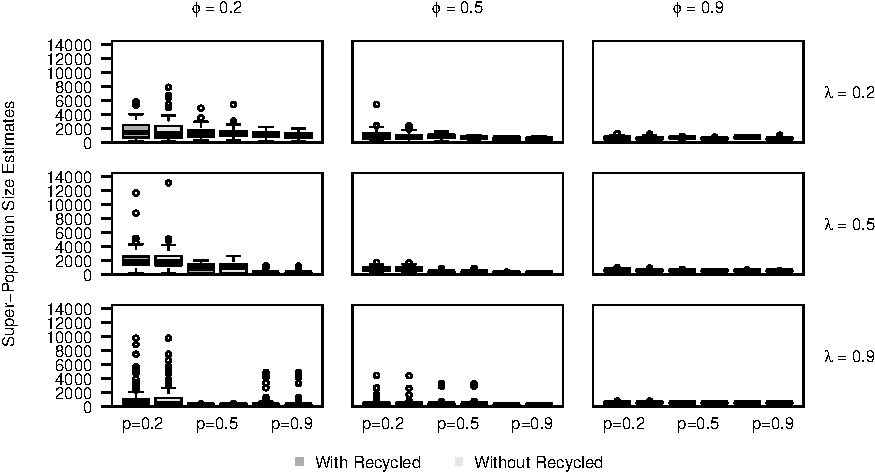
\includegraphics{Appendix_BW_files/figure-latex/figure23_superN_GJSTL5-1.pdf}

\textsc{Web Figure 23:} Boxplots of super-population size estimates
(\(N\)) of 100 simulated datasets analyzed with and without the effect
of recycled individuals for population size \(1000\) with \(T_2=1\) for
5 sample times for varying survival (\(\phi=0.2,0.5,0.9\)), capture
(\(p=0.2,0.5,0.9\)), and tag retention (\(\lambda=0.2,0.5,0.9\))
probabilities. The black line indicates the true value of \(N\) used to
simulate the data for each model.

\paragraph{N=1000, T=0.5, t=7}\label{n1000-t0.5-t7}

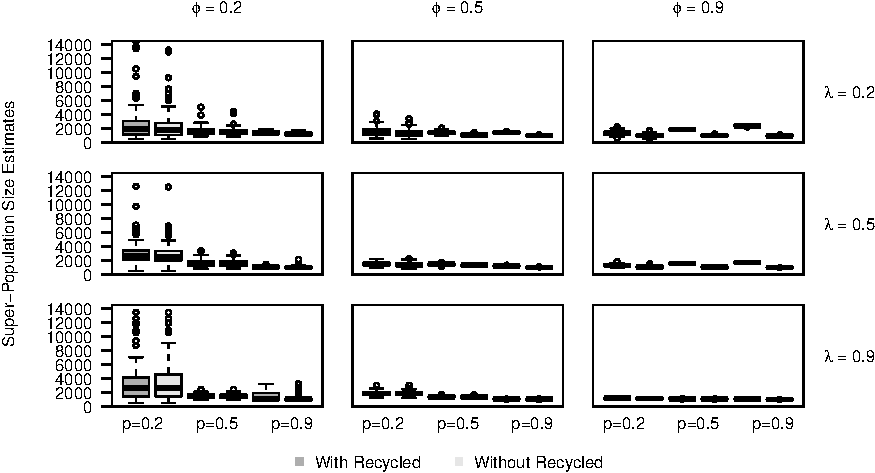
\includegraphics{Appendix_BW_files/figure-latex/figure24_superN_GJSTL6-1.pdf}

\textsc{Web Figure 24:} Boxplots of super-population size estimates
(\(N\)) of 100 simulated datasets analyzed with and without the effect
of recycled individuals for population size \(1000\) with \(T_2=1\) for
7 sample times for varying survival (\(\phi=0.2,0.5,0.9\)), capture
(\(p=0.2,0.5,0.9\)), and tag retention (\(\lambda=0.2,0.5,0.9\))
probabilities. The black line indicates the true value of \(N\) used to
simulate the data for each model.

\newpage

\subsection{Abundance Estimates}\label{abundance-estimates}

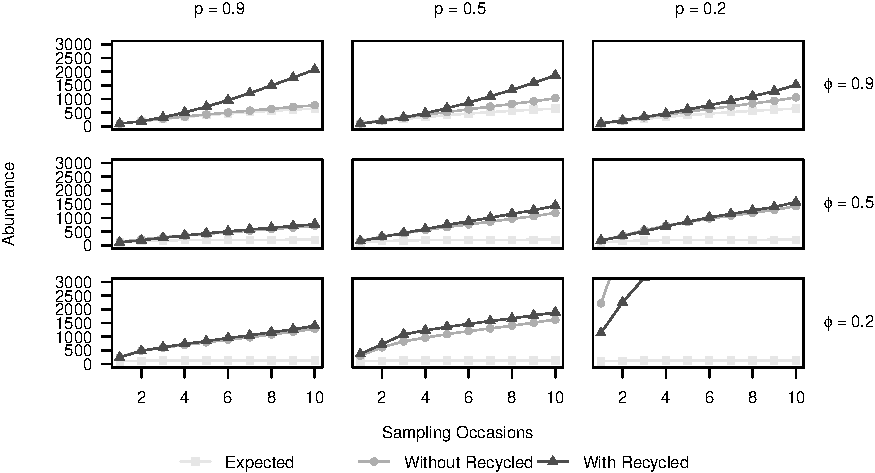
\includegraphics{Appendix_BW_files/figure-latex/25_abundance_L_GJSTL1-1.pdf}

\textsc{Web Figure 25:} Mean abundance estimates (\(N_j\)'s) for each
sample time (\(k=10\)) between analysis with and without recycled
individuals with population size \(N=1000\) with \(T_2=1\) with 10 sample times for low tag retention (\(\lambda=0.2\)), varying survival
probabilities (\(\phi=0.2,0.5,0.9\)) and varying capture probabilities
(\(p=0.2,0.5,0.9\)).

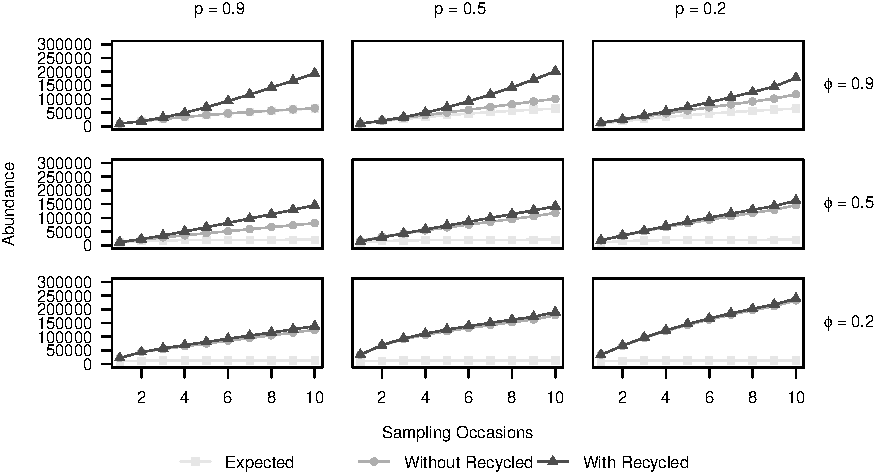
\includegraphics{Appendix_BW_files/figure-latex/26_abundance_L_GJSTL2-1.pdf}

\textsc{Web Figure 26:} Mean abundance estimates (\(N_j\)'s) for each
sample time (\(k=10\)) between analysis with and without recycled
individuals with population size \(N=100000\) with \(T_2=1\) with 10
sample times for low tag retention (\(\lambda=0.2\)), varying survival
probabilities (\(\phi=0.2,0.5,0.9\)) and varying capture probabilities
(\(p=0.2,0.5,0.9\)).

\newpage

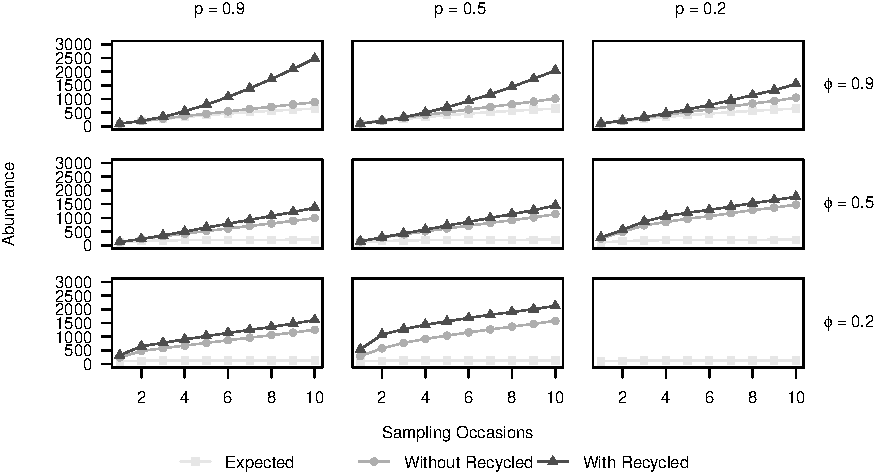
\includegraphics{Appendix_BW_files/figure-latex/27_abundance_L_GJSTL4-1.pdf}

\textsc{Web Figure 27:} Mean abundance estimates (\(N_j\)'s) for each
sample time (\(k=10\)) between analysis with and without recycled
individuals with population size \(N=1000\) with \(T_2=0.5\) with 10
sample times for low tag retention (\(\lambda=0.2\)), varying survival
probabilities (\(\phi=0.2,0.5,0.9\)) and varying capture probabilities
(\(p=0.2,0.5,0.9\)).

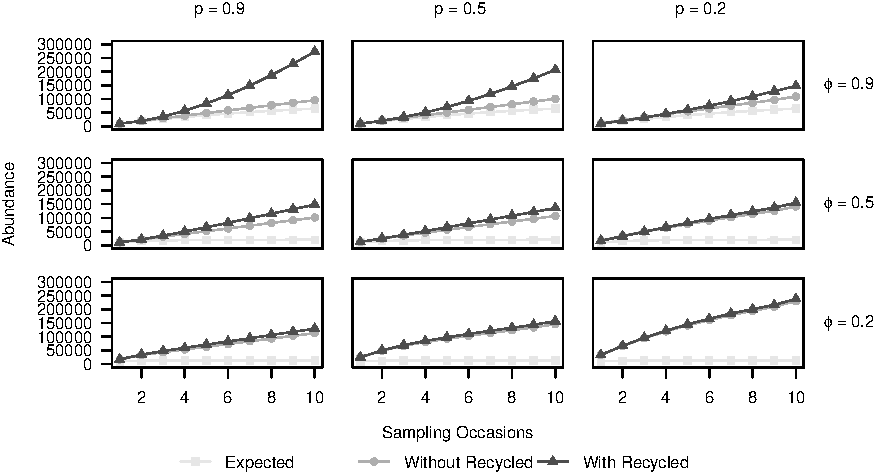
\includegraphics{Appendix_BW_files/figure-latex/28_abundance_L_GJSTL3-1.pdf}

\textsc{Web Figure 28:} Mean abundance estimates (\(N_j\)'s) for each
sample time (\(k=10\)) between analysis with and without recycled
individuals with population size \(N=100000\) with \(T_2=0.5\) with 10
sample times for low tag retention (\(\lambda=0.2\)), varying survival
probabilities (\(\phi=0.2,0.5,0.9\)) and varying capture probabilities
(\(p=0.2,0.5,0.9\)).

\newpage

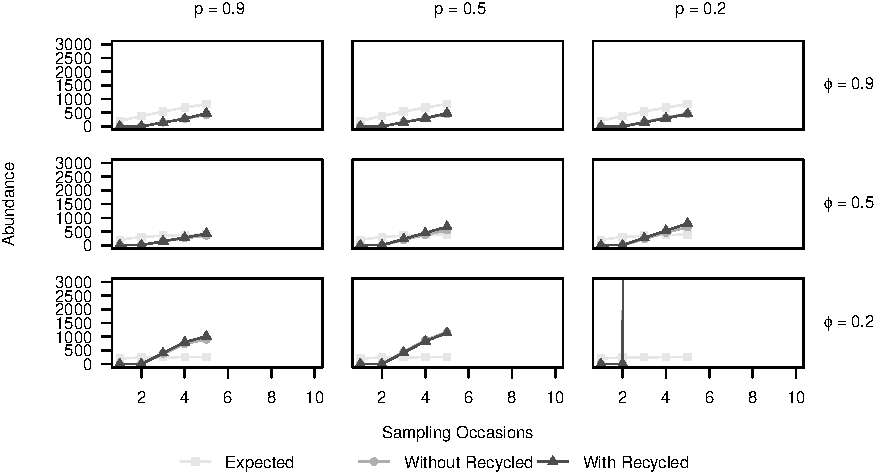
\includegraphics{Appendix_BW_files/figure-latex/29_abundance_L_GJSTL5-1.pdf}

\textsc{Web Figure 29:} Mean abundance estimates (\(N_j\)'s) for each
sample time (\(k=5\)) between analysis with and without recycled
individuals with population size \(N=1000\) with \(T_2=1\) with 5 sample times for low tag retention (\(\lambda=0.2\)), varying survival
probabilities (\(\phi=0.2,0.5,0.9\)) and varying capture probabilities
(\(p=0.2,0.5,0.9\)).

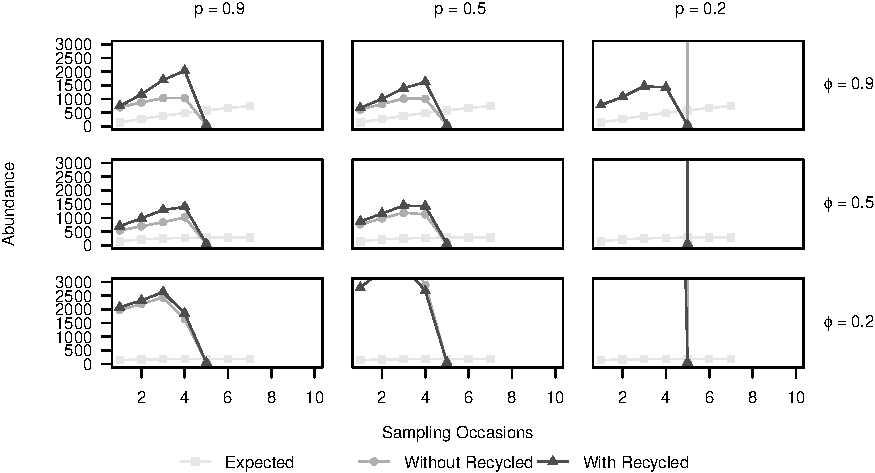
\includegraphics{Appendix_BW_files/figure-latex/30_abundance_L_GJSTL6-1.pdf}

\textsc{Web Figure 30:} Mean abundance estimates (\(N_j\)'s) for each
sample time (\(k=7\)) between analysis with and without recycled
individuals with population size \(N=1000\) with \(T_2=1\) with 7 sample times
for low tag retention (\(\lambda=0.2\)), varying survival
probabilities (\(\phi=0.2,0.5,0.9\)) and varying capture probabilities
(\(p=0.2,0.5,0.9\)).

\newpage

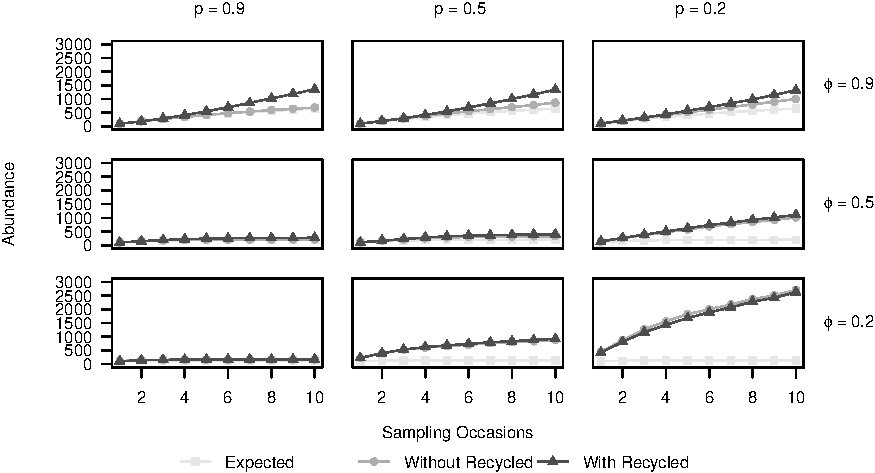
\includegraphics{Appendix_BW_files/figure-latex/31_abundance_M_GJSTL1-1.pdf}

\textsc{Web Figure 31:} Mean abundance estimates (\(N_j\)'s) for each
sample time (\(k=10\)) between analysis with and without recycled
individuals with population size \(N=1000\) with \(T_2=1\) with 10 sample times
for medium tag retention (\(\lambda=0.5\)), varying survival
probabilities (\(\phi=0.2,0.5,0.9\)) and varying capture probabilities
(\(p=0.2,0.5,0.9\)).

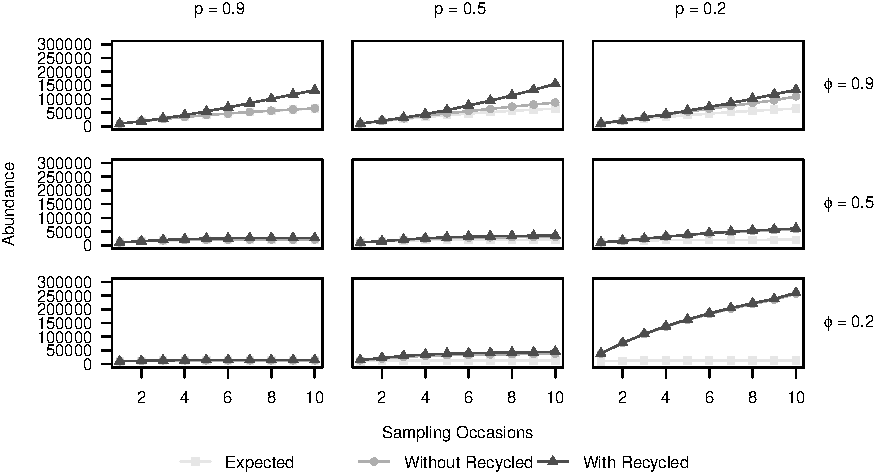
\includegraphics{Appendix_BW_files/figure-latex/32_abundance_M_GJSTL2-1.pdf}

\textsc{Web Figure 32:} Mean abundance estimates (\(N_j\)'s) for each
sample time (\(k=10\)) between analysis with and without recycled
individuals with population size \(N=100000\) with \(T_2=1\) with 10
sample times for medium tag retention (\(\lambda=0.5\)), varying
survival probabilities (\(\phi=0.2,0.5,0.9\)) and varying capture
probabilities (\(p=0.2,0.5,0.9\)).

\newpage

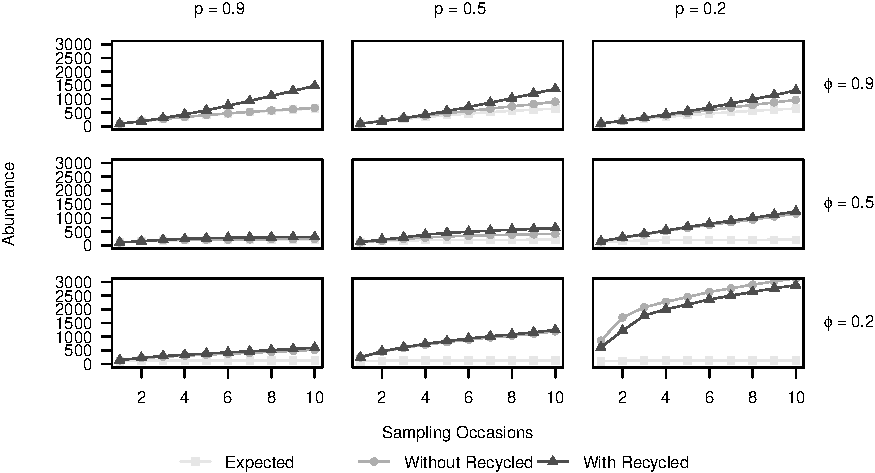
\includegraphics{Appendix_BW_files/figure-latex/33_abundance_M_GJSTL4-1.pdf}

\textsc{Web Figure 33:} Mean abundance estimates (\(N_j\)'s) for each
sample time (\(k=10\)) between analysis with and without recycled
individuals with population size \(N=1000\) with \(T_2=0.5\) with 10
sample times for medium tag retention (\(\lambda=0.5\)), varying
survival probabilities (\(\phi=0.2,0.5,0.9\)) and varying capture
probabilities (\(p=0.2,0.5,0.9\)).

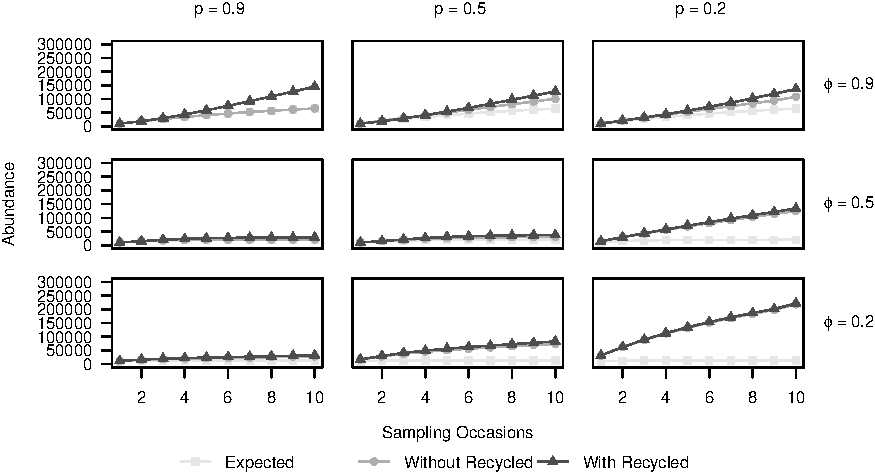
\includegraphics{Appendix_BW_files/figure-latex/34_abundance_M_GJSTL3-1.pdf}

\textsc{Web Figure 34:} Mean abundance estimates (\(N_j\)'s) for each
sample time (\(k=10\)) between analysis with and without recycled
individuals with population size \(N=100000\) with \(T_2=0.5\) with 10
sample times for medium tag retention (\(\lambda=0.5\)), varying
survival probabilities (\(\phi=0.2,0.5,0.9\)) and varying capture
probabilities (\(p=0.2,0.5,0.9\)).

\newpage

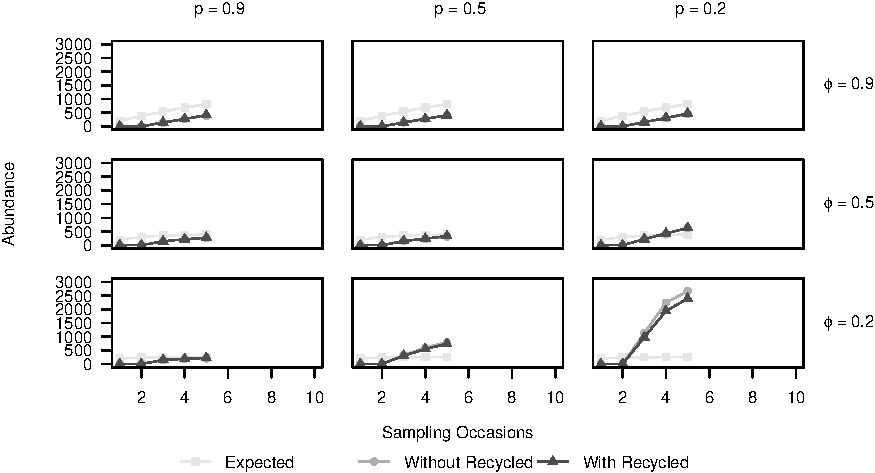
\includegraphics{Appendix_BW_files/figure-latex/35_abundance_M_GJSTL5-1.pdf}

\textsc{Web Figure 35:} Mean abundance estimates (\(N_j\)'s) for each
sample time (\(k=5\)) between analysis with and without recycled
individuals with population size \(N=1000\) with \(T_2=1\) with 5 sample times
for medium tag retention (\(\lambda=0.5\)), varying survival
probabilities (\(\phi=0.2,0.5,0.9\)) and varying capture probabilities
(\(p=0.2,0.5,0.9\)).

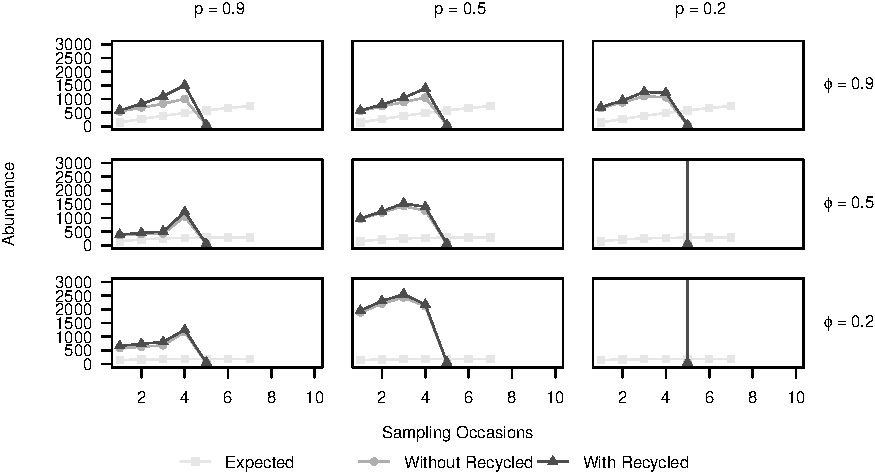
\includegraphics{Appendix_BW_files/figure-latex/36_abundance_M_GJSTL6-1.pdf}

\textsc{Web Figure 36:} Mean abundance estimates (\(N_j\)'s) for each
sample time (\(k=7\)) between analysis with and without recycled
individuals with population size \(N=1000\) with \(T_2=1\) with 7 sample times for medium tag retention (\(\lambda=0.5\)), varying survival
probabilities (\(\phi=0.2,0.5,0.9\)) and varying capture probabilities
(\(p=0.2,0.5,0.9\)).

\newpage

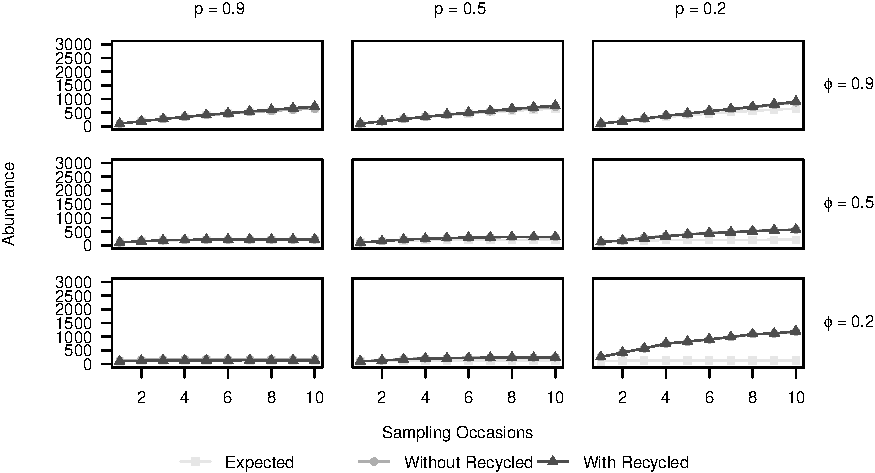
\includegraphics{Appendix_BW_files/figure-latex/37_abundance_H_GJSTL1-1.pdf}

\textsc{Web Figure 37:} Mean abundance estimates (\(N_j\)'s) for each
sample time (\(k=10\)) between analysis with and without recycled
individuals with population size \(N=1000\) with \(T_2=1\) with 10 sample times for high tag retention (\(\lambda=0.9\)), varying survival
probabilities (\(\phi=0.2,0.5,0.9\)) and varying capture probabilities
(\(p=0.2,0.5,0.9\)).

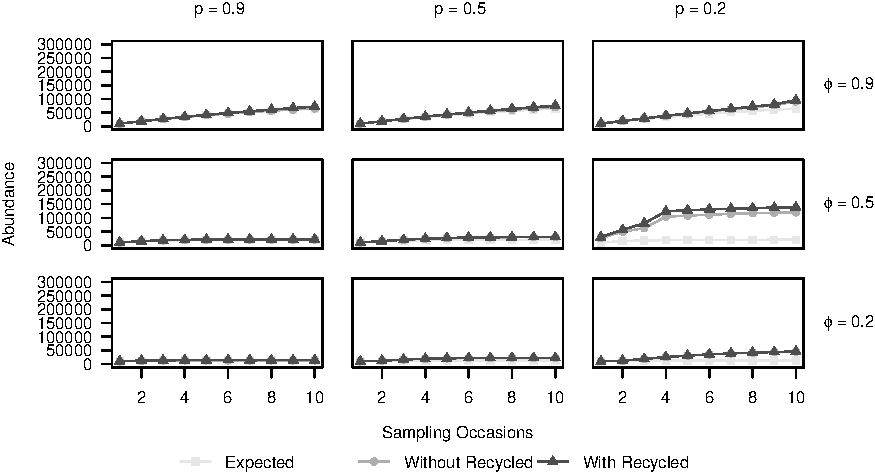
\includegraphics{Appendix_BW_files/figure-latex/38_abundance_H_GJSTL2-1.pdf}

\textsc{Web Figure 38:} Mean abundance estimates (\(N_j\)'s) for each
sample time (\(k=10\)) between analysis with and without recycled
individuals with population size \(N=100000\) with \(T_2=1\) with 10
sample times for high tag retention (\(\lambda=0.9\)), varying survival
probabilities (\(\phi=0.2,0.5,0.9\)) and varying capture probabilities
(\(p=0.2,0.5,0.9\)).

\newpage

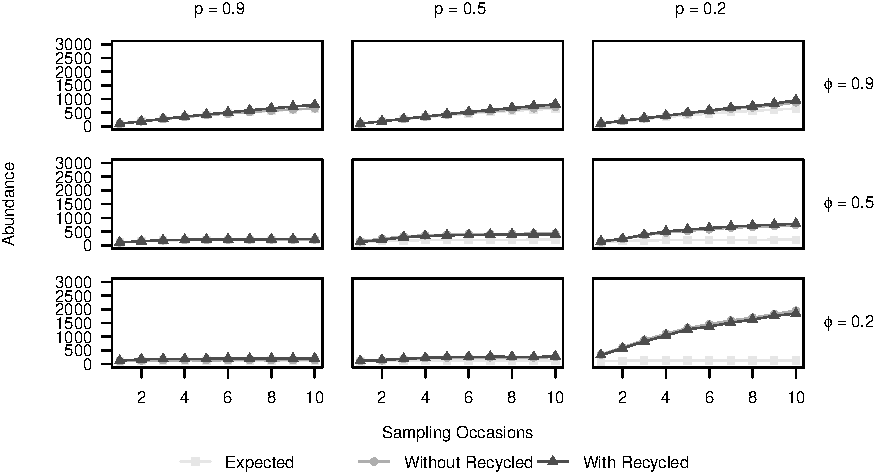
\includegraphics{Appendix_BW_files/figure-latex/39_abundance_H_GJSTL4-1.pdf}

\textsc{Web Figure 39:} Mean abundance estimates (\(N_j\)'s) for each
sample time (\(k=10\)) between analysis with and without recycled
individuals with population size \(N=1000\) with \(T_2=0.5\) with 10
sample times for high tag retention (\(\lambda=0.9\)), varying survival
probabilities (\(\phi=0.2,0.5,0.9\)) and varying capture probabilities
(\(p=0.2,0.5,0.9\)).

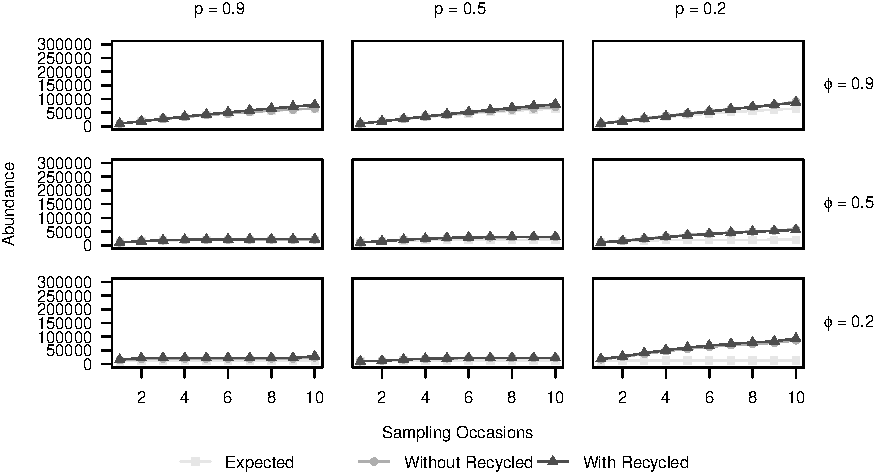
\includegraphics{Appendix_BW_files/figure-latex/40_abundance_H_GJSTL3-1.pdf}

\textsc{Web Figure 40:} Mean abundance estimates (\(N_j\)'s) for each
sample time (\(k=10\)) between analysis with and without recycled
individuals with population size \(N=100000\) with \(T_2=0.5\) with 10
sample times for high tag retention (\(\lambda=0.9\)), varying survival
probabilities (\(\phi=0.2,0.5,0.9\)) and varying capture probabilities
(\(p=0.2,0.5,0.9\)).

\newpage

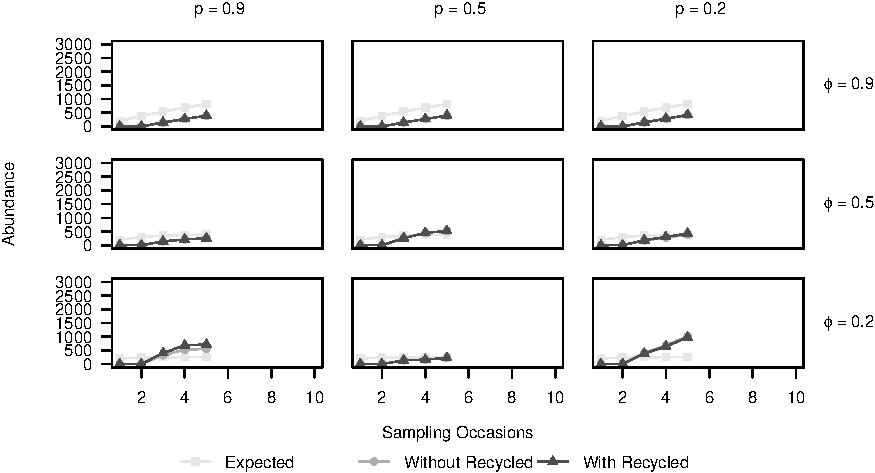
\includegraphics{Appendix_BW_files/figure-latex/41_abundance_H_GJSTL5-1.pdf}

\textsc{Web Figure 41:} Mean abundance estimates (\(N_j\)'s) for each
sample time (\(k=5\)) between analysis with and without recycled
individuals with population size \(N=1000\) with \(T_2=1\) with 5 sample times for high tag retention (\(\lambda=0.9\)), varying survival
probabilities (\(\phi=0.2,0.5,0.9\)) and varying capture probabilities
(\(p=0.2,0.5,0.9\)).

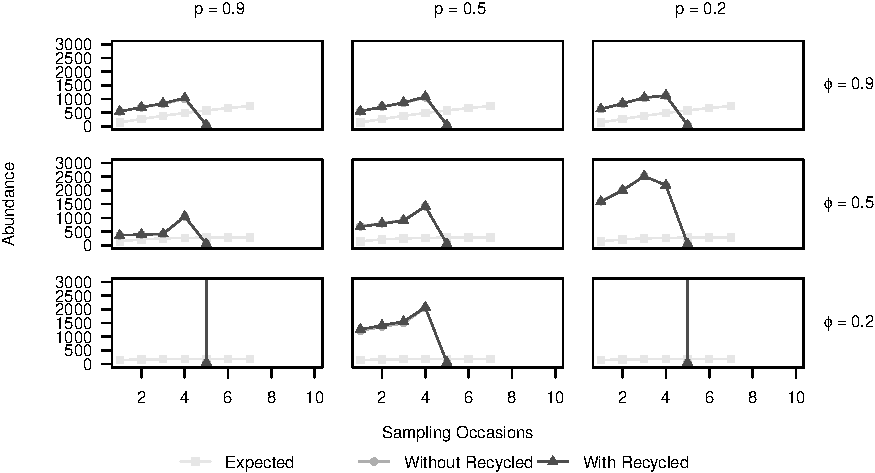
\includegraphics{Appendix_BW_files/figure-latex/42_abundance_H_GJSTL6-1.pdf}

\textsc{Web Figure 42:} Mean abundance estimates (\(N_j\)'s) for each
sample time (\(k=7\)) between analysis with and without recycled
individuals with population size \(N=1000\) with \(T_2=1\) with 5 sample times for high tag retention (\(\lambda=0.9\)), varying survival
probabilities (\(\phi=0.2,0.5,0.9\)) and varying capture probabilities
(\(p=0.2,0.5,0.9\)).

\newpage

\subsection{Recycled Individuals}\label{recycled-individuals}

\textsc{Web Table 17:} Examples of the fraction of recycled individuals
(number of recycled individuals captured / total number of individuals
captured) at each sample time for a 10 sample-time experiment with
super-population size \(N=1000\) with 100\% double-tagging.

\begin{table}[ht]
\begin{tabular}{rrrrrrrrrrr}
  \hline
& \multicolumn{10}{c}{Sampling Times}\\
 & 1 & 2 & 3 & 4 & 5 & 6 & 7 & 8 & 9 & 10 \\ 
  \hline
  $\phi=0.9, p=0.9, \lambda=0.2$ & 0.00 & 0.30 & 0.36 & 0.47 & 0.51 & 0.53 & 0.54 & 0.55 & 0.56 & 0.57 \\ 
  $\phi=0.9, p=0.9, \lambda=0.5$ & 0.00 & 0.12 & 0.12 & 0.20 & 0.29 & 0.26 & 0.29 & 0.30 & 0.31 & 0.31 \\ 
  $\phi=0.9, p=0.9, \lambda=0.9$ & 0.00 & 0.01 & 0.02 & 0.02 & 0.01 & 0.01 & 0.03 & 0.04 & 0.04 & 0.03 \\ \hline
  $\phi=0.9, p=0.5, \lambda=0.2$ & 0.00 & 0.14 & 0.28 & 0.38 & 0.43 & 0.48 & 0.54 & 0.54 & 0.55 & 0.56 \\ 
  $\phi=0.9, p=0.5, \lambda=0.5$ & 0.00 & 0.02 & 0.12 & 0.14 & 0.27 & 0.28 & 0.28 & 0.33 & 0.29 & 0.38 \\ 
  $\phi=0.9, p=0.5, \lambda=0.9$ & 0.00 & 0.00 & 0.00 & 0.00 & 0.01 & 0.02 & 0.02 & 0.04 & 0.06 & 0.06 \\ \hline
  $\phi=0.9, p=0.2, \lambda=0.2$ & 0.00 & 0.05 & 0.15 & 0.35 & 0.18 & 0.28 & 0.30 & 0.33 & 0.40 & 0.37 \\ 
  $\phi=0.9, p=0.2, \lambda=0.5$ & 0.00 & 0.00 & 0.06 & 0.09 & 0.14 & 0.13 & 0.20 & 0.21 & 0.30 & 0.26 \\ 
  $\phi=0.9, p=0.2, \lambda=0.9$ & 0.00 & 0.00 & 0.00 & 0.00 & 0.00 & 0.01 & 0.02 & 0.02 & 0.04 & 0.03 \\ \hline
  $\phi=0.5, p=0.9, \lambda=0.2$ & 0.00 & 0.18 & 0.23 & 0.27 & 0.34 & 0.36 & 0.32 & 0.32 & 0.32 & 0.26 \\ 
  $\phi=0.5, p=0.9, \lambda=0.5$ & 0.00 & 0.10 & 0.10 & 0.15 & 0.10 & 0.15 & 0.18 & 0.13 & 0.19 & 0.12 \\ 
  $\phi=0.5, p=0.9, \lambda=0.9$ & 0.00 & 0.00 & 0.00 & 0.01 & 0.01 & 0.00 & 0.01 & 0.01 & 0.01 & 0.01 \\ \hline
  $\phi=0.2, p=0.9, \lambda=0.2$ & 0.00 & 0.10 & 0.14 & 0.07 & 0.15 & 0.10 & 0.11 & 0.13 & 0.13 & 0.12 \\ 
  $\phi=0.2, p=0.9, \lambda=0.5$ & 0.00 & 0.02 & 0.06 & 0.05 & 0.05 & 0.11 & 0.04 & 0.06 & 0.08 & 0.09 \\ 
  $\phi=0.2, p=0.9, \lambda=0.9$ & 0.00 & 0.01 & 0.00 & 0.01 & 0.00 & 0.00 & 0.00 & 0.00 & 0.00 & 0.00 \\ \hline
    $\phi=0.5, p=0.5, \lambda=0.5$ & 0.00 & 0.01 & 0.07 & 0.06 & 0.12 & 0.13 & 0.14 & 0.16 & 0.13 & 0.14 \\ \hline
\end{tabular}
\end{table}

\textsc{Web Table 18:} Examples of the fraction of recycled individuals
(number of recycled individuals captured / total number of individuals
captured) at each sample time for a 7 sample-time experiment with
super-population size \(N=1000\) with 100\% double-tagging.

\begin{table}[ht]
\begin{tabular}{rrrrrrrr}
  \hline
  & \multicolumn{7}{c}{Sampling Times}\\
 & 1 & 2 & 3 & 4 & 5 & 6 & 7 \\ 
  \hline
  $\phi=0.9, p=0.9, \lambda=0.2$ & 0.00 & 0.32 & 0.40 & 0.49 & 0.50 & 0.53 & 0.55 \\ 
  $\phi=0.9, p=0.9, \lambda=0.5$ & 0.00 & 0.10 & 0.18 & 0.21 & 0.22 & 0.29 & 0.29 \\ 
  $\phi=0.9, p=0.9, \lambda=0.9$ & 0.00 & 0.01 & 0.01 & 0.02 & 0.02 & 0.02 & 0.02 \\ \hline
  $\phi=0.9, p=0.5, \lambda=0.2$ & 0.00 & 0.12 & 0.30 & 0.35 & 0.42 & 0.47 & 0.50 \\ 
  $\phi=0.9, p=0.5, \lambda=0.5$ & 0.00 & 0.06 & 0.15 & 0.22 & 0.26 & 0.24 & 0.27 \\ 
  $\phi=0.9, p=0.5, \lambda=0.9$ & 0.00 & 0.01 & 0.00 & 0.02 & 0.02 & 0.03 & 0.04 \\ \hline
  $\phi=0.9, p=0.2, \lambda=0.2$ & 0.00 & 0.05 & 0.12 & 0.15 & 0.22 & 0.21 & 0.30 \\ 
  $\phi=0.9, p=0.2, \lambda=0.5$ & 0.00 & 0.00 & 0.06 & 0.10 & 0.15 & 0.20 & 0.20 \\ 
  $\phi=0.9, p=0.2, \lambda=0.9$ & 0.00 & 0.00 & 0.00 & 0.00 & 0.00 & 0.01 & 0.01 \\ \hline
  $\phi=0.5, p=0.9, \lambda=0.2$ & 0.00 & 0.19 & 0.30 & 0.32 & 0.30 & 0.34 & 0.38 \\ 
  $\phi=0.5, p=0.9, \lambda=0.5$ & 0.00 & 0.09 & 0.12 & 0.13 & 0.15 & 0.11 & 0.14 \\ 
  $\phi=0.5, p=0.9, \lambda=0.9$ & 0.00 & 0.00 & 0.00 & 0.02 & 0.00 & 0.00 & 0.01 \\ \hline
  $\phi=0.2, p=0.9, \lambda=0.2$ & 0.00 & 0.10 & 0.11 & 0.12 & 0.13 & 0.16 & 0.08 \\ 
  $\phi=0.2, p=0.9, \lambda=0.5$ & 0.00 & 0.04 & 0.05 & 0.07 & 0.07 & 0.03 & 0.02 \\ 
  $\phi=0.2, p=0.9, \lambda=0.2$ & 0.00 & 0.00 & 0.00 & 0.00 & 0.00 & 0.00 & 0.00 \\ \hline
    $\phi=0.5, p=0.5, \lambda=0.5$ & 0.00 & 0.05 & 0.04 & 0.05 & 0.09 & 0.11 & 0.12 \\ \hline
\end{tabular}
\end{table}

\clearpage

\textsc{Web Table 19:} Examples of the fraction of recycled individuals
(number of recycled individuals captured / total number of individuals
captured) at each sample time for a 5 sample-time experiment with
super-population size \(N=1000\) with 100\% double-tagging.

\begin{table}[ht]
\begin{tabular}{rrrrrr}
  \hline
  & \multicolumn{5}{c}{Sampling Times}\\
 & 1 & 2 & 3 & 4 & 5 \\ 
  \hline
 $\phi=0.9, p=0.9, \lambda=0.2$  & 0.00 & 0.29 & 0.34 & 0.45 & 0.52 \\ 
  $\phi=0.9, p=0.9, \lambda=0.5$  & 0.00 & 0.08 & 0.22 & 0.23 & 0.28 \\ 
  $\phi=0.9, p=0.9, \lambda=0.9$  & 0.00 & 0.01 & 0.01 & 0.02 & 0.02 \\ \hline 
  $\phi=0.9, p=0.5, \lambda=0.2$  & 0.00 & 0.14 & 0.27 & 0.33 & 0.38 \\ 
  $\phi=0.9, p=0.5, \lambda=0.5$  & 0.00 & 0.05 & 0.13 & 0.18 & 0.25 \\ 
  $\phi=0.9, p=0.5, \lambda=0.9$  & 0.00 & 0.00 & 0.01 & 0.01 & 0.02 \\ \hline
  $\phi=0.9, p=0.2, \lambda=0.2$  & 0.00 & 0.06 & 0.15 & 0.16 & 0.29 \\ 
  $\phi=0.9, p=0.2, \lambda=0.5$ & 0.00 & 0.03 & 0.06 & 0.08 & 0.12 \\ 
  $\phi=0.9, p=0.2, \lambda=0.9$ & 0.00 & 0.00 & 0.00 & 0.01 & 0.01 \\ \hline
  $\phi=0.5, p=0.9, \lambda=0.2$ & 0.00 & 0.14 & 0.25 & 0.30 & 0.33 \\ 
  $\phi=0.5, p=0.9, \lambda=0.5$ & 0.00 & 0.05 & 0.13 & 0.10 & 0.15 \\ 
  $\phi=0.5, p=0.9, \lambda=0.9$ & 0.00 & 0.00 & 0.01 & 0.01 & 0.00 \\ \hline
  $\phi=0.2, p=0.9, \lambda=0.2$ & 0.00 & 0.11 & 0.10 & 0.13 & 0.12 \\ 
  $\phi=0.2, p=0.9, \lambda=0.5$  & 0.00 & 0.02 & 0.03 & 0.05 & 0.04 \\ 
  $\phi=0.2, p=0.9, \lambda=0.9$  & 0.00 & 0.00 & 0.00 & 0.00 & 0.00 \\ \hline
    $\phi=0.5, p=0.5, \lambda=0.5$ & 0.00 & 0.03 & 0.09 & 0.10 & 0.12 \\ \hline
\end{tabular}
\end{table}


\end{document}
